% !TeX document-id = {d7247aab-0d3b-456c-a2ca-7facee9734c0}
% !TeX encoding = utf8
% !TeX program = xelatex
% !BIB program = bibtex
%

\documentclass[german,pg]{tudo-sse-thesis}

% Provide your title
\title{Entwicklung eines 3D RPG Videospiels mittels prozeduraler Inhaltsgenerieung und Deep Reinforcement Learning}

% Provide your name
\author{Jan Beier, Nils Dunker, Leonard Fricke, Niklas Haldorn, Kay Heider, \linebreak Jona Lukas Heinrichs, Mathieu Herkersdorf, Carsten Kellner, Markus Mügge, Thomas Rysch, Jannik Stadtler, Tom Voellmer}

\firstexaminer{Marco Pleines}
\secondexaminer{Nicolas Fischöder}
\thirdexaminer{Prof. Dr. Günter Rudolph}

\usepackage{amsmath}				% Mathematischer Formelsatz AMS
\usepackage{amsfonts}

\usepackage[autostyle,german=guillemets,german=quotes]{csquotes}
\usepackage{todonotes}

\usepackage{tikz-qtree}
\usepackage{tikz}
\usetikzlibrary{shapes,arrows,arrows.meta,automata,positioning,fit,calc,matrix,backgrounds}
\usepackage{algorithmic}
\usepackage{subcaption}
\renewcommand{\algorithmicrequire}{\textbf{Eingabe:}}
\renewcommand{\algorithmicensure}{\textbf{Ausgabe:}}
\usepackage{mathtools}
\usepackage{gensymb}
\usepackage{siunitx}
\usepackage[german]{algorithm2e}				% Algorithmen Umgebung mit Algorithmenverzeichnis
\renewcommand{\listalgorithmcfname}{Algorithmenverzeichnis}
\usepackage{listings}
\usepackage{ulem}					% Unterstreichen von Text
\usepackage{color}					% Farben wenn es sein muß
\usepackage{hyperref}				% Klickbare Verweise und \autoref{label}
\usepackage{booktabs}				% "Schöne" Tabellen	
\usepackage{minted}

% Custom-Liste für Themenallokation
\usepackage{enumitem}
\newlist{thallok}{enumerate}{10}
\setlist[thallok]{label*=\arabic*.}


\begin{document}
	
	\maketitle
	
	\pagenumbering{roman}

	\tableofcontents
	\cleardoublepage
	
	\pagenumbering{arabic}
	
	\chapter{Einleitung}

\section{Motivation und Problemstellung}

Die prozedurale Generierung von NPCs sowie das Erlernen von Bewegungen und das Animieren dieser stellt heutzutage in der Videospielindustrie eine zentrale Herausforderung dar. Nicht nur müssen Kreaturen effizient und somit oftmals zur Laufzeit generiert werden, sondern es müssen auch die Animationen welche durch maschinelles Lernen erlernt werden, auf ein möglichst breites Spektrum an Kreaturen anwendbar sein. Dabei ist es also essentiell, dass das Training der Kreaturen möglichst generalisiert stattfindet, sodass bei der Kreatur-Generierung eine große, sich bei den Körpermerkmalen variierende Menge der Kreaturen erzeugt werden kann, wodurch weniger Einschränkungen für die Körpereigenschaften der NPCs aufkommen. Somit sollten also die Animationen auf einen möglichst breiten Pool von Kreaturen anwendbar sein, ohne für zufällig erzeugte, potentiell neue, Körpermerkmale neu trainieren zu müssen.

Weiterhin muss bei der Generierung von Spielfiguren die relevante Herausforderung des automatischen Aufspannens eines Meshes über den bis zu diesem Zeitpunkt untexturierten Körper einer Kreatur gelöst werden; das sogenannte \textit{Automatic Rigging}, welches ebenfalls zu dem prozeduralen Erzeugen von Kreaturen dazugehört. Es muss also hier das relevante Problem betrachtet werden, Meshes welche ggf. ebenfalls prozedural erzeugt werden, auf das breite Spektrum von verschiedenen Körperausprägungen des Kreaturen-Pools anwenden zu können, ohne dass es zu sehr von den Körperformen der Kreaturen abweicht \textcolor{red}{text, da sonst die Dreiecksnetze degenerieren und nachfolgende numerische Operationen fehlschlagen würden.? Oder bereits zu technisch?}

Ferner könnte die prozedurale Generierung von Inhalten in einem Videospiel nicht nur zum Erzeugen von Kreaturen zum Einsatz kommen, sondern auch für die Spielwelt selbst. Damit könnte ... \textcolor{red}{Notiz für Thomas: Sobald Inhalte von World-Generation stehen, hier ein wenig ausführen.}


  ... mesh muss zu creature passen... lernen der bewegung anpassbar bezüglich creature-pool

\section{Zielsetzung und Vorgehensweise}
\label{Zielsetzung_und_Vorgehensweise}

Bei der Entwicklung eines Spieles müssen viele Themengebiete zur Planung einkalkuliert werden, um während der Entwicklung eine Übersicht zu behalten und das Endziel stets zu berücksichtigen. Daher wurde sich für die Einteilung des Spieldesigns in folgende verschiedene Bereiche entschieden, an welchen parallel gearbeitet werden kann: die Generierung von Spielleveln, die Evaluation der generierten Level, Generierung der Monster, Fortbewegung der Monster und zuletzt die Strategie bzw. Verhaltensweise der Monster. Innerhalb jeder dieser Bereiche sollen bestimmte Anforderungen erfüllt sein: \newline \newline
\textbf{\textit{Die Generierung von Spielleveln}}\newline
\begin{itemize}
	\item Die Generierung der Spiellevel sollte prozedural durchgeführt werden: z.B. durch KD-Trees, L-Systeme, Space-Partitioning
	\item Die Spiellevel enthalten Böden, Wände und auch Spawn-Points für Objekte und NPCs
	\item Gleichzeitig sollen die Komplexität, Größe und der Schwierigkeitsgrad der Level parametrisierbar sein
\end{itemize}
\textbf{\textit{Evaluation der Generierten Level}}
\begin{itemize}
	\item Die Level/Spielwelten sollen anhand vorbestimmter Metriken evaluiert werden, wie z.B.: Lösbarkeit der Level, Schwierigkeitsgrad
	\item Folgende Ansätze sind dafür vorgeschlagen: Imitation Learning, Deep Reinforcement Learning
\end{itemize}
\textbf{\textit{Generierung der Monster}}
\begin{itemize}
	\item In diesem Bereich sind viele Freiheiten gelassen worden, da die Generierung der Monster auf viele unterschiedliche Weisen durchgeführt werden kann
	\item Relevant dabei ist nur, dass die Erstellung von NPCs algorithmus-basiert ist und dass innerhalb von Unity die von Unity bereitgestellten Joints verwendet werden sollten
	\item Eine Orientierungshilfe dabei kann der Unity-ML-Agents-Walker sein
\end{itemize}
\textbf{\textit{Fortbewegung der Monster}}
\begin{itemize}
	\item Animationen sollen nicht händisch erstellt werden
	\item Die Monster sollen sich mit Hilfe von Deep Reinforcement Learning lernen zu bewegen
	\item Der Agent wählt die Kräfte aus, welche auf seine Joints ausgeübt werden
	\item Je nach lösen einer spezifischen Aufgabe wird der Agent dann belohnt
	\item Dabei könnten Inverse Kinematiken nützlich sein
\end{itemize}
\textbf{\textit{Strategie bzw. Verhaltensweise der Monster}}
\begin{itemize}
	\item Klassische Ansätze (high level) wären hier die Behavior Trees oder auch State machines
	\item Währenddessen lernende Ansätze (low level) wären Imitation Learning und Deep Reinforcement learning
\end{itemize}

Ein besonderer Schwerpunkt soll dabei auf die Themen der \textbf{Generierung der Monster} und der \textbf{Fortbewegung der Monster} gelegt werden, da diese die Basis für die restlichen Aufgaben bilden sollten. Es wurde sich absichtlich dafür entschieden von Anfang an kein klares Design der späteren Spielwelt, Monster und des Spielercharakters zu definieren, sodass sich daraus keine Einschränkungen für die initiale Implementierungsphase ergeben sollten. Vielmehr wurde entschieden die Entwicklung des Creature-Generation Tools abzuwarten, sodass mit der Fertigstellung anhand der Stärken des Tools das Spieldesign abgeleitet werden kann. Damit dieser Grundstein gelegt werden konnte, wurde sich dafür entschieden die \textbf{Generierung der Monster} und die \textbf{Fortbewegung der Monster} der Spielwelt als erstes zu priorisieren und somit die 12 Teilnehmer der Projektgruppe für die Anfangsphase in zwei Untergruppen aufzuteilen: die \textbf{Creature-Generator}, bestehend aus 7 Mitgliedern, und die \textbf{Creature-Animator}, bestehend aus 5 Mitgliedern. Es wird antizipiert, dass sich mit fortschreitender Zeit die Gruppen, sobald die Basis für das Spiel besteht, in weitere (kleinere) Gruppen aufteilen werden. Das Ziel ist somit, parallel an mehreren Themen gleichzeitig arbeiten zu können und somit effizient Fortschritt zu machen. Währenddessen muss eine deutliche Kommunikation zwischen den (Unter-)Gruppen bestehen um die Themen miteinander abstimmen zu können, vor allem für die Anfangsphase zwischen den \textbf{Creature-Generator} und den \textbf{Creature-Animator}.

Für diese Anfangsphase wurde evaluiert, die Kreatur-Generierung so einfach wie möglich zu halten um das Beibringen von Bewegungen durch die \textbf{Creature-Animator} Gruppe so einfach wie möglich zu gestalten und die Freiheitsgrade auf einem Minimum zu halten. Dafür ist das Vorhaben zweibeinige, humanoide Kreaturen und auch vierbeinige Kreaturen erzeugen zu können. Zusätzliche Körperteile wie beispielsweise Flügel, mehrere Arme oder Beine und Ähnliche Extras werden weggelassen, damit keine zusätzlichen Freiheitsgrade hinzukommen und das Lernen der Bewegung der Kreatur gegebenenfalls erschweren würden. Trotzdem soll später evaluiert werden, ob solche ergänzenden Körperteile hinzugefügt werden könnten, sobald die Basisstruktur, also das stabile Erzeugen und Lernen der Bewegungen der Kreaturen, besteht. Außerdem wird durch diesen Ansatz der Spielentwurf so schlicht wie möglich gehalten, sodass keine potentiellen Einschränkungen bezüglich des Spieldesigns existieren und damit die spätere Gestaltung des Spiels basierend auf den dann bestehenden Funktionalitäten entschieden werden kann. 

Zur Erzeugung der Geometrie für generierte Kreaturen haben wir eine neue Methode basierend auf Metaballs (siehe Abschnitt \ref{sec:metaball}) entwickelt, die das Mesh aus mehreren deformierbaren Kapseln zusammensetzt. Dabei werden die Probleme von vorherigen Methoden umgangen, die durch das zusammensetzen aus zu vielen Kugeln entstehen und das Mesh schwer kontrollierbar machen.



\section{Übersicht}

Zunächst werden in dem Kapitel \ref{Grundlagen} alle Grundlagen beschrieben in Bezug auf die angeführten Themenbereiche der Projektgruppe welche in der Seminarphase gegenseitig vorgestellt wurden \ref{Zielsetzung_und_Vorgehensweise}. Basierend auf diesen Themengebieten werden dann in Kapitel \ref{Verwandte_Arbeiten} verwandte Arbeiten und Literatur vorgestellt, welche sowohl während der Evaluation in der Seminarphase erforscht wurden, als auch in der späteren Erarbeitung weiterer Themen und Algorithmen (Kapitel \ref{ch:projektorganisation} und \ref{Technische_Umsetzung}) ausgemacht wurden. Sobald die Grundlagen über die Themen der späteren fachlichen und technischen Vorgehensweise geklärt sind, wird in Kapitel \ref{ch:projektorganisation} die Entscheidungsgrundlage für die organisatorische Vorgehensweise beschrieben, welches sich während der Entwicklungsphase der verschiedenen Bereiche \ref{Zielsetzung_und_Vorgehensweise} erschlossen hat. Nachdem das organisatorische Prozedere bekannt ist, wird im Anschluss die fachliche Vorgehensweise und die Umsetzung in Kapitel \ref{Technische_Umsetzung} evaluiert. Anschließend werden in Kapitel \ref{Vorlaeufige_Ergebnisse} die Ergebnisse präsentiert und diskutiert in Kapitel \ref{Diskussion}. Schließlich wird in Kapitel \ref{Ausblick} zusammengefasst, auf welche (Forschungs-)Bereiche die Erkenntnisse dieser Studie ausgeweitet werden können.
	
	\chapter{Grundlagen}

(Die benutzten) Vortragsthemen vom Anfang hier als eigene Unterkapitel beschreiben.

%  Grundlagen L-System: Allgemein, Theoretischer Hintergrund, 2D, 3D
\section{L-System}
Eine zentrale Eigenschaft in der Natur ist die Selbstähnlichkeit von Strukturen auf makroskopischer und mikroskopischer Ebene~\cite{Shaker2016}. % ref this + reword
Hier lassen sich dieselben Strukturen in verschiedenen Größenordnungen wiederfinden. % delete this
Beispielsweise ähneln die Knospen eines Blumenkohls auch seiner äußeren Struktur, wie in Abbildung~\ref{fig:Blumenkohl}\footnote{Quelle: {https://commons.wikimedia.org/wiki/File:Blumenkohl-1.jpg}, Autor: Rainer Zenz, CC BY-SA 3.0 <http://creativecommons.org/licenses/by-sa/3.0/>, via Wikimedia Commons} zu sehen ist.
\begin{figure}[ht]
    \centering
    \includegraphics[width=0.5\linewidth]{chapters/02_Grundlagen/L_System/Blumenkohl-1.jpg}
    \caption{Blumenkohl}\label{fig:Blumenkohl}
\end{figure}

Um diese Eigenschaften präzise und strukturell darzustellen kann ein Lindenmayer-System (L-System)~\cite{lindenmayer1990} eingesetzt werden.
Die Basis eines L-Systems bildet eine kontextfreie Grammatik $G=(N,T,S,P)$ mit einer Menge von Nicht-Terminalsymbolen $N$, Terminalsymbolen $T$, einem Startsymbol $S$ und einer Menge von Produktionen $P$.
Der Unterschied zwischen einem L-System und einer üblichen kontextfreien Grammatik besteht darin, dass in einem Ableitungsschritt eines L-Systems parallel alle Nicht-Terminale ersetzt werden.
Zusätzlich werden nur eine feste Anzahl an Ableitungsschritten durchgeführt und es kann anstatt eines Startsymbols auch ein Startstring angegeben werden.

\subsection{Grafische Darstellung in 2D}
Der resultierende String einer Ableitung kann grafisch als Zeichenvorschriften für \emph{turtle graphics} gesehen werden. % reword
In \emph{turtle graphics} gibt es eine \emph{turtle}, oder Zeichenkopf, der initial in eine Richtung zeigt und sich in zwei oder drei Dimensionen fortbewegen kann.
Bei jeder Fortbewegung wird entlang der aktuellen Richtung des Kopfes und der hinterlegten Distanz eine Strecke gezeichnet.
Die Symbole der Grammatik werden hierbei als Fortbewegung um eine gewisse Distanz oder eine Drehung um eine der Achsen interpretiert.
In Abbildung~\ref{fig:L-System 2D Rotation} ist eine Visualisierung dieses Konzeptes zu sehen.
Hier ist der Zeichenkopf initial nach oben gerichtet.
% Add 2D rotation tikz
\begin{figure}[ht]
    \centering
    % \resizebox{\linewidth-3cm}{!}{%
        
    % }
    \includegraphics[width=0.5\linewidth]{example-image-a}
    \caption{L-System 2D Rotation}\label{fig:L-System 2D Rotation}
\end{figure}

Ohne Erweiterungen entstehen hierbei immer zusammenhängende Strukturen bei dem der Zeichenkopf nicht springen kann.
Das heißt, Blätter oder Äste sind nur schwer zu realisieren.


\subsection{Erweiterungen}
Damit komplexere Strukturen abgebildet werden können, werden zusätzliche Symbole eingesetzt und die Auswertung erweitert.
Zwei übliche Erweiterung die besonders zur Generierung von Vegetation nützlich sind, sind \emph{Bracketed L-Systeme} und \emph{Stochastische L-Systeme}.

\subsubsection{Bracketed L-Systeme}
Um Strukturen abzubilden die nur durch "absetzen" des Stiftes generiert werden können, können \emph{Bracketed L-Systeme}~\cite*{Shaker2016} eingesetzt werden.
Damit die generierte Struktur zusammenhängend bleibt, wird die Position und aktuelle Richtung des Zeichenkopfes auf einem Stack gespeichert und kann durch \texttt{push} und \texttt{pop} Operationen verwaltet werden.
Die Menge der Nicht-Terminalsymbole wird dabei um \texttt{[} für die \texttt{push} Operation und \texttt{]} für \texttt{pop} erweitert.

Mit dieser Erweiterung können nun auch Äste von Bäumen oder Stängel von Blumen gezeichnet werden.
Ein Beispiel für eine Art von Strauch kann mittels dieses L-Systems erzeugt werden:
\begin{itemize}
    \item Nicht-Terminalsymbole $N=\{F\}$
    \item Terminalsymbole $T=\{\texttt{+},\texttt{-},\texttt{[},\texttt{]}\}$
    \item Startstring $S=F$
    \item Produktionen:
    \begin{align*}
        F\rightarrow~F\texttt{[+}F\texttt{]}F\texttt{[-}F\texttt{]}\texttt{[}F\texttt{]}
    \end{align*}
\end{itemize}

Hierbei beschreibt das Nicht-Terminalsymbol $F$ eine Fortbewegung, \texttt{+} und \texttt{-} jeweils eine Drehung um 30 Grad nach links bzw. rechts in 2D und \texttt{[}, \texttt{]} beschreiben die \texttt{push} und \texttt{pop} Operationen.
Die generierten Strukturen sind in Abbildung~\ref{fig:Bracketed} zu sehen.

\begin{figure}[ht]
    \begin{subfigure}[t]{.3\textwidth}
        \centering
        \resizebox{!}{100px}{\begin{tikzpicture}\draw (0,0) -- (0,0);
\draw (0,0) -- (0,10);
\draw (0,10) -- (-5,19);
\draw (0,10) -- (0,10);
\draw (0,10) -- (0,20);
\draw (0,20) -- (5,29);
\draw (0,20) -- (0,20);
\draw (0,20) -- (0,30);
\draw (0,20) -- (0,20);
\end{tikzpicture}}

        \caption*{1 Ableitungsschritt}
    \end{subfigure}
    \hfill
    \begin{subfigure}[t]{.3\textwidth}
        \centering
        \resizebox{!}{100bp}{\begin{tikzpicture}\draw (0,0) -- (0,0);
\draw (0,0) -- (0,10);
\draw (0,10) -- (-5,19);
\draw (0,10) -- (0,10);
\draw (0,10) -- (0,20);
\draw (0,20) -- (5,29);
\draw (0,20) -- (0,20);
\draw (0,20) -- (0,30);
\draw (0,20) -- (0,20);
\draw (0,20) -- (-5,29);
\draw (-5,29) -- (-14,34);
\draw (-5,29) -- (-5,29);
\draw (-5,29) -- (-10,38);
\draw (-10,38) -- (-10,48);
\draw (-10,38) -- (-10,38);
\draw (-10,38) -- (-15,47);
\draw (-10,38) -- (-10,38);
\draw (0,20) -- (0,20);
\draw (0,20) -- (0,30);
\draw (0,30) -- (-5,39);
\draw (0,30) -- (0,30);
\draw (0,30) -- (0,40);
\draw (0,40) -- (5,49);
\draw (0,40) -- (0,40);
\draw (0,40) -- (0,50);
\draw (0,40) -- (0,40);
\draw (0,40) -- (5,49);
\draw (5,49) -- (5,59);
\draw (5,49) -- (5,49);
\draw (5,49) -- (10,58);
\draw (10,58) -- (19,63);
\draw (10,58) -- (10,58);
\draw (10,58) -- (15,67);
\draw (10,58) -- (10,58);
\draw (0,40) -- (0,40);
\draw (0,40) -- (0,50);
\draw (0,50) -- (-5,59);
\draw (0,50) -- (0,50);
\draw (0,50) -- (0,60);
\draw (0,60) -- (5,69);
\draw (0,60) -- (0,60);
\draw (0,60) -- (0,70);
\draw (0,60) -- (0,60);
\draw (0,40) -- (0,40);
\end{tikzpicture}}

        \caption*{2 Ableitungsschritte}
    \end{subfigure}
    \hfill
    \begin{subfigure}[t]{.3\textwidth}
        \centering
        \resizebox{!}{100bp}{\begin{tikzpicture}\draw (0,0) -- (0,0);
\draw (0,0) -- (0,10);
\draw (0,10) -- (-5,19);
\draw (0,10) -- (0,10);
\draw (0,10) -- (0,20);
\draw (0,20) -- (5,29);
\draw (0,20) -- (0,20);
\draw (0,20) -- (0,30);
\draw (0,20) -- (0,20);
\draw (0,20) -- (-5,29);
\draw (-5,29) -- (-14,34);
\draw (-5,29) -- (-5,29);
\draw (-5,29) -- (-10,38);
\draw (-10,38) -- (-10,48);
\draw (-10,38) -- (-10,38);
\draw (-10,38) -- (-15,47);
\draw (-10,38) -- (-10,38);
\draw (0,20) -- (0,20);
\draw (0,20) -- (0,30);
\draw (0,30) -- (-5,39);
\draw (0,30) -- (0,30);
\draw (0,30) -- (0,40);
\draw (0,40) -- (5,49);
\draw (0,40) -- (0,40);
\draw (0,40) -- (0,50);
\draw (0,40) -- (0,40);
\draw (0,40) -- (5,49);
\draw (5,49) -- (5,59);
\draw (5,49) -- (5,49);
\draw (5,49) -- (10,58);
\draw (10,58) -- (19,63);
\draw (10,58) -- (10,58);
\draw (10,58) -- (15,67);
\draw (10,58) -- (10,58);
\draw (0,40) -- (0,40);
\draw (0,40) -- (0,50);
\draw (0,50) -- (-5,59);
\draw (0,50) -- (0,50);
\draw (0,50) -- (0,60);
\draw (0,60) -- (5,69);
\draw (0,60) -- (0,60);
\draw (0,60) -- (0,70);
\draw (0,60) -- (0,60);
\draw (0,40) -- (0,40);
\draw (0,40) -- (-5,49);
\draw (-5,49) -- (-14,54);
\draw (-5,49) -- (-5,49);
\draw (-5,49) -- (-10,58);
\draw (-10,58) -- (-10,68);
\draw (-10,58) -- (-10,58);
\draw (-10,58) -- (-15,67);
\draw (-10,58) -- (-10,58);
\draw (-10,58) -- (-19,63);
\draw (-19,63) -- (-29,63);
\draw (-19,63) -- (-19,63);
\draw (-19,63) -- (-28,68);
\draw (-28,68) -- (-33,77);
\draw (-28,68) -- (-28,68);
\draw (-28,68) -- (-37,73);
\draw (-28,68) -- (-28,68);
\draw (-10,58) -- (-10,58);
\draw (-10,58) -- (-15,67);
\draw (-15,67) -- (-24,72);
\draw (-15,67) -- (-15,67);
\draw (-15,67) -- (-20,76);
\draw (-20,76) -- (-20,86);
\draw (-20,76) -- (-20,76);
\draw (-20,76) -- (-25,85);
\draw (-20,76) -- (-20,76);
\draw (-20,76) -- (-20,86);
\draw (-20,86) -- (-25,95);
\draw (-20,86) -- (-20,86);
\draw (-20,86) -- (-20,96);
\draw (-20,96) -- (-15,105);
\draw (-20,96) -- (-20,96);
\draw (-20,96) -- (-20,106);
\draw (-20,96) -- (-20,96);
\draw (-20,76) -- (-20,76);
\draw (-20,76) -- (-25,85);
\draw (-25,85) -- (-34,90);
\draw (-25,85) -- (-25,85);
\draw (-25,85) -- (-30,94);
\draw (-30,94) -- (-30,104);
\draw (-30,94) -- (-30,94);
\draw (-30,94) -- (-35,103);
\draw (-30,94) -- (-30,94);
\draw (-20,76) -- (-20,76);
\draw (0,40) -- (0,40);
\draw (0,40) -- (0,50);
\draw (0,50) -- (-5,59);
\draw (0,50) -- (0,50);
\draw (0,50) -- (0,60);
\draw (0,60) -- (5,69);
\draw (0,60) -- (0,60);
\draw (0,60) -- (0,70);
\draw (0,60) -- (0,60);
\draw (0,60) -- (-5,69);
\draw (-5,69) -- (-14,74);
\draw (-5,69) -- (-5,69);
\draw (-5,69) -- (-10,78);
\draw (-10,78) -- (-10,88);
\draw (-10,78) -- (-10,78);
\draw (-10,78) -- (-15,87);
\draw (-10,78) -- (-10,78);
\draw (0,60) -- (0,60);
\draw (0,60) -- (0,70);
\draw (0,70) -- (-5,79);
\draw (0,70) -- (0,70);
\draw (0,70) -- (0,80);
\draw (0,80) -- (5,89);
\draw (0,80) -- (0,80);
\draw (0,80) -- (0,90);
\draw (0,80) -- (0,80);
\draw (0,80) -- (5,89);
\draw (5,89) -- (5,99);
\draw (5,89) -- (5,89);
\draw (5,89) -- (10,98);
\draw (10,98) -- (19,103);
\draw (10,98) -- (10,98);
\draw (10,98) -- (15,107);
\draw (10,98) -- (10,98);
\draw (0,80) -- (0,80);
\draw (0,80) -- (0,90);
\draw (0,90) -- (-5,99);
\draw (0,90) -- (0,90);
\draw (0,90) -- (0,100);
\draw (0,100) -- (5,109);
\draw (0,100) -- (0,100);
\draw (0,100) -- (0,110);
\draw (0,100) -- (0,100);
\draw (0,80) -- (0,80);
\draw (0,80) -- (5,89);
\draw (5,89) -- (5,99);
\draw (5,89) -- (5,89);
\draw (5,89) -- (10,98);
\draw (10,98) -- (19,103);
\draw (10,98) -- (10,98);
\draw (10,98) -- (15,107);
\draw (10,98) -- (10,98);
\draw (10,98) -- (10,108);
\draw (10,108) -- (5,117);
\draw (10,108) -- (10,108);
\draw (10,108) -- (10,118);
\draw (10,118) -- (15,127);
\draw (10,118) -- (10,118);
\draw (10,118) -- (10,128);
\draw (10,118) -- (10,118);
\draw (10,98) -- (10,98);
\draw (10,98) -- (15,107);
\draw (15,107) -- (15,117);
\draw (15,107) -- (15,107);
\draw (15,107) -- (20,116);
\draw (20,116) -- (29,121);
\draw (20,116) -- (20,116);
\draw (20,116) -- (25,125);
\draw (20,116) -- (20,116);
\draw (20,116) -- (29,121);
\draw (29,121) -- (34,130);
\draw (29,121) -- (29,121);
\draw (29,121) -- (38,126);
\draw (38,126) -- (48,126);
\draw (38,126) -- (38,126);
\draw (38,126) -- (47,131);
\draw (38,126) -- (38,126);
\draw (20,116) -- (20,116);
\draw (20,116) -- (25,125);
\draw (25,125) -- (25,135);
\draw (25,125) -- (25,125);
\draw (25,125) -- (30,134);
\draw (30,134) -- (39,139);
\draw (30,134) -- (30,134);
\draw (30,134) -- (35,143);
\draw (30,134) -- (30,134);
\draw (20,116) -- (20,116);
\draw (0,80) -- (0,80);
\draw (0,80) -- (0,90);
\draw (0,90) -- (-5,99);
\draw (0,90) -- (0,90);
\draw (0,90) -- (0,100);
\draw (0,100) -- (5,109);
\draw (0,100) -- (0,100);
\draw (0,100) -- (0,110);
\draw (0,100) -- (0,100);
\draw (0,100) -- (-5,109);
\draw (-5,109) -- (-14,114);
\draw (-5,109) -- (-5,109);
\draw (-5,109) -- (-10,118);
\draw (-10,118) -- (-10,128);
\draw (-10,118) -- (-10,118);
\draw (-10,118) -- (-15,127);
\draw (-10,118) -- (-10,118);
\draw (0,100) -- (0,100);
\draw (0,100) -- (0,110);
\draw (0,110) -- (-5,119);
\draw (0,110) -- (0,110);
\draw (0,110) -- (0,120);
\draw (0,120) -- (5,129);
\draw (0,120) -- (0,120);
\draw (0,120) -- (0,130);
\draw (0,120) -- (0,120);
\draw (0,120) -- (5,129);
\draw (5,129) -- (5,139);
\draw (5,129) -- (5,129);
\draw (5,129) -- (10,138);
\draw (10,138) -- (19,143);
\draw (10,138) -- (10,138);
\draw (10,138) -- (15,147);
\draw (10,138) -- (10,138);
\draw (0,120) -- (0,120);
\draw (0,120) -- (0,130);
\draw (0,130) -- (-5,139);
\draw (0,130) -- (0,130);
\draw (0,130) -- (0,140);
\draw (0,140) -- (5,149);
\draw (0,140) -- (0,140);
\draw (0,140) -- (0,150);
\draw (0,140) -- (0,140);
\draw (0,120) -- (0,120);
\draw (0,80) -- (0,80);
\end{tikzpicture}}

        \caption*{3 Ableitungsschritte}
    \end{subfigure}
    \caption{Resultate bracketed L-System}\label{fig:Bracketed}
\end{figure}


\subsubsection{Stochastische L-Systeme}
Eine Eigenschaft von den bisher verwendeten L-Systemen ist, dass die Produktionen deterministisch ausgewertet werden.
Um realistische Pflanzen generieren zu können muss jedoch etwas Variation eingeführt werden; es wäre also vorteilhaft, wenn die Produktionen nicht-deterministisch ausgewertet werden.
Dazu kann ein \emph{stochastisches L-System}~\cite*{Shaker2016} verwendet werden.
Hierbei kann es mehrere Produktionen mit gleichen linken Seiten geben.
Jeweils über die Menge von Produktionen mit gleicher linken Seite wird eine Wahrscheinlichkeitsverteilung erstellt.
Das heißt die Auswahl der Ersetzung eines Nicht-Terminalsymbols erfolgt zufällig.

Im Folgenden ist ein Beispiel für ein stochastisches bracketed L-System gegeben:
\begin{itemize}
    \item Nicht-Terminalsymbole $N=\{F\}$
    \item Terminalsymbole $T=\{\texttt{+},\texttt{-},\texttt{[},\texttt{]}\}$
    \item Startstring $S=F$
    \item Produktionen:
    \begin{align*}
        F\xrightarrow{0.33} & ~F\texttt{[+}F\texttt{]}F\texttt{[-}F\texttt{]} F \\
        F\xrightarrow{0.33} & ~F\texttt{[+}F\texttt{]} F                         \\
        F\xrightarrow{0.34} & ~F\texttt{[-}F\texttt{]} F
    \end{align*}
\end{itemize}

Hier gibt es für das Nicht-Terminal $F$ drei Produktionen, zwei Produktionen mit einer Wahrscheinlichkeit von $33\%$ gewählt und eine Produktion mit $34\%$.
Drei resultierende Bilder dieses L-Systems sind in Abbildung~\ref{fig:Stochastic} gegeben.
Hieran kann man gut sehen wie aus einem L-System deutlich unterschiedliche Strukturen generiert werden können die jedoch alle ähnliche Grundstrukturen aufweisen.
\begin{figure}[ht]
    \begin{subfigure}[t]{.25\textwidth}
        \centering
        \resizebox{!}{175px}{\begin{tikzpicture}\draw (0,0) -- (0,0);
\draw (0,0) -- (0,10);
\draw (0,10) -- (-5,19);
\draw (0,10) -- (0,10);
\draw (0,10) -- (0,20);
\draw (0,20) -- (5,29);
\draw (5,29) -- (5,39);
\draw (5,29) -- (5,29);
\draw (5,29) -- (10,38);
\draw (0,20) -- (0,20);
\draw (0,20) -- (0,30);
\draw (0,30) -- (-5,39);
\draw (0,30) -- (0,30);
\draw (0,30) -- (0,40);
\draw (0,40) -- (5,49);
\draw (5,49) -- (14,54);
\draw (5,49) -- (5,49);
\draw (5,49) -- (10,58);
\draw (10,58) -- (10,68);
\draw (10,68) -- (5,77);
\draw (10,68) -- (10,68);
\draw (10,68) -- (10,78);
\draw (10,58) -- (10,58);
\draw (10,58) -- (15,67);
\draw (15,67) -- (15,77);
\draw (15,67) -- (15,67);
\draw (15,67) -- (20,76);
\draw (0,40) -- (0,40);
\draw (0,40) -- (0,50);
\draw (0,50) -- (5,59);
\draw (0,50) -- (0,50);
\draw (0,50) -- (0,60);
\draw (0,60) -- (-5,69);
\draw (0,60) -- (0,60);
\draw (0,60) -- (0,70);
\draw (0,70) -- (5,79);
\draw (5,79) -- (5,89);
\draw (5,79) -- (5,79);
\draw (5,79) -- (10,88);
\draw (0,70) -- (0,70);
\draw (0,70) -- (0,80);
\draw (0,80) -- (5,89);
\draw (0,80) -- (0,80);
\draw (0,80) -- (0,90);
\draw (0,90) -- (-5,99);
\draw (0,90) -- (0,90);
\draw (0,90) -- (0,100);
\draw (0,100) -- (-5,109);
\draw (-5,109) -- (-5,119);
\draw (-5,109) -- (-5,109);
\draw (-5,109) -- (-10,118);
\draw (-10,118) -- (-19,123);
\draw (-10,118) -- (-10,118);
\draw (-10,118) -- (-15,127);
\draw (-15,127) -- (-15,137);
\draw (-15,137) -- (-10,146);
\draw (-15,137) -- (-15,137);
\draw (-15,137) -- (-15,147);
\draw (-15,127) -- (-15,127);
\draw (-15,127) -- (-20,136);
\draw (-20,136) -- (-20,146);
\draw (-20,136) -- (-20,136);
\draw (-20,136) -- (-25,145);
\draw (-25,145) -- (-34,150);
\draw (-34,150) -- (-44,150);
\draw (-34,150) -- (-34,150);
\draw (-34,150) -- (-43,155);
\draw (-25,145) -- (-25,145);
\draw (-25,145) -- (-30,154);
\draw (-30,154) -- (-30,164);
\draw (-30,154) -- (-30,154);
\draw (-30,154) -- (-35,163);
\draw (-35,163) -- (-44,168);
\draw (-35,163) -- (-35,163);
\draw (-35,163) -- (-40,172);
\draw (0,100) -- (0,100);
\draw (0,100) -- (0,110);
\draw (0,110) -- (-5,119);
\draw (0,110) -- (0,110);
\draw (0,110) -- (0,120);
\draw (0,120) -- (-5,129);
\draw (-5,129) -- (-5,139);
\draw (-5,129) -- (-5,129);
\draw (-5,129) -- (-10,138);
\draw (-10,138) -- (-19,143);
\draw (-10,138) -- (-10,138);
\draw (-10,138) -- (-15,147);
\draw (0,120) -- (0,120);
\draw (0,120) -- (0,130);
\draw (0,130) -- (5,139);
\draw (0,130) -- (0,130);
\draw (0,130) -- (0,140);
\draw (0,140) -- (-5,149);
\draw (0,140) -- (0,140);
\draw (0,140) -- (0,150);
\draw (0,150) -- (5,159);
\draw (5,159) -- (14,164);
\draw (5,159) -- (5,159);
\draw (5,159) -- (10,168);
\draw (10,168) -- (10,178);
\draw (10,168) -- (10,168);
\draw (10,168) -- (15,177);
\draw (15,177) -- (24,182);
\draw (24,182) -- (29,191);
\draw (24,182) -- (24,182);
\draw (24,182) -- (33,187);
\draw (15,177) -- (15,177);
\draw (15,177) -- (20,186);
\draw (20,186) -- (29,191);
\draw (20,186) -- (20,186);
\draw (20,186) -- (25,195);
\draw (25,195) -- (25,205);
\draw (25,205) -- (30,214);
\draw (25,205) -- (25,205);
\draw (25,205) -- (25,215);
\draw (25,215) -- (20,224);
\draw (25,215) -- (25,215);
\draw (25,215) -- (25,225);
\draw (25,225) -- (30,234);
\draw (30,234) -- (39,239);
\draw (30,234) -- (30,234);
\draw (30,234) -- (35,243);
\draw (35,243) -- (35,253);
\draw (35,243) -- (35,243);
\draw (35,243) -- (40,252);
\draw (25,225) -- (25,225);
\draw (25,225) -- (25,235);
\draw (25,235) -- (20,244);
\draw (25,235) -- (25,235);
\draw (25,235) -- (25,245);
\draw (25,245) -- (20,254);
\draw (20,254) -- (20,264);
\draw (20,254) -- (20,254);
\draw (20,254) -- (15,263);
\draw (25,245) -- (25,245);
\draw (25,245) -- (25,255);
\draw (25,255) -- (30,264);
\draw (25,255) -- (25,255);
\draw (25,255) -- (25,265);
\draw (25,265) -- (20,274);
\draw (25,265) -- (25,265);
\draw (25,265) -- (25,275);
\draw (25,195) -- (25,195);
\draw (25,195) -- (30,204);
\draw (30,204) -- (30,214);
\draw (30,204) -- (30,204);
\draw (30,204) -- (35,213);
\draw (35,213) -- (35,223);
\draw (35,223) -- (30,232);
\draw (35,223) -- (35,223);
\draw (35,223) -- (35,233);
\draw (35,213) -- (35,213);
\draw (35,213) -- (40,222);
\draw (40,222) -- (49,227);
\draw (40,222) -- (40,222);
\draw (40,222) -- (45,231);
\draw (45,231) -- (45,241);
\draw (45,231) -- (45,231);
\draw (45,231) -- (50,240);
\draw (0,150) -- (0,150);
\draw (0,150) -- (0,160);
\draw (0,160) -- (-5,169);
\draw (0,160) -- (0,160);
\draw (0,160) -- (0,170);
\draw (0,170) -- (5,179);
\draw (5,179) -- (14,184);
\draw (5,179) -- (5,179);
\draw (5,179) -- (10,188);
\draw (10,188) -- (10,198);
\draw (10,188) -- (10,188);
\draw (10,188) -- (15,197);
\draw (0,170) -- (0,170);
\draw (0,170) -- (0,180);
\draw (0,180) -- (-5,189);
\draw (0,180) -- (0,180);
\draw (0,180) -- (0,190);
\draw (0,190) -- (5,199);
\draw (5,199) -- (14,204);
\draw (5,199) -- (5,199);
\draw (5,199) -- (10,208);
\draw (10,208) -- (10,218);
\draw (10,208) -- (10,208);
\draw (10,208) -- (15,217);
\draw (15,217) -- (24,222);
\draw (24,222) -- (29,231);
\draw (24,222) -- (24,222);
\draw (24,222) -- (33,227);
\draw (15,217) -- (15,217);
\draw (15,217) -- (20,226);
\draw (20,226) -- (29,231);
\draw (20,226) -- (20,226);
\draw (20,226) -- (25,235);
\draw (25,235) -- (25,245);
\draw (25,245) -- (30,254);
\draw (25,245) -- (25,245);
\draw (25,245) -- (25,255);
\draw (25,235) -- (25,235);
\draw (25,235) -- (30,244);
\draw (30,244) -- (39,249);
\draw (30,244) -- (30,244);
\draw (30,244) -- (35,253);
\draw (0,190) -- (0,190);
\draw (0,190) -- (0,200);
\draw (0,200) -- (5,209);
\draw (0,200) -- (0,200);
\draw (0,200) -- (0,210);
\draw (0,210) -- (-5,219);
\draw (0,210) -- (0,210);
\draw (0,210) -- (0,220);
\draw (0,220) -- (5,229);
\draw (5,229) -- (14,234);
\draw (5,229) -- (5,229);
\draw (5,229) -- (10,238);
\draw (0,220) -- (0,220);
\draw (0,220) -- (0,230);
\draw (0,230) -- (5,239);
\draw (0,230) -- (0,230);
\draw (0,230) -- (0,240);
\draw (0,240) -- (-5,249);
\draw (0,240) -- (0,240);
\draw (0,240) -- (0,250);
\draw (0,250) -- (-5,259);
\draw (-5,259) -- (-14,264);
\draw (-5,259) -- (-5,259);
\draw (-5,259) -- (-10,268);
\draw (-10,268) -- (-19,273);
\draw (-19,273) -- (-24,282);
\draw (-19,273) -- (-19,273);
\draw (-19,273) -- (-28,278);
\draw (-10,268) -- (-10,268);
\draw (-10,268) -- (-15,277);
\draw (-15,277) -- (-15,287);
\draw (-15,277) -- (-15,277);
\draw (-15,277) -- (-20,286);
\draw (-20,286) -- (-29,291);
\draw (-20,286) -- (-20,286);
\draw (-20,286) -- (-25,295);
\draw (-25,295) -- (-25,305);
\draw (-25,305) -- (-20,314);
\draw (-25,305) -- (-25,305);
\draw (-25,305) -- (-25,315);
\draw (-25,315) -- (-30,324);
\draw (-25,315) -- (-25,315);
\draw (-25,315) -- (-25,325);
\draw (-25,325) -- (-30,334);
\draw (-30,334) -- (-30,344);
\draw (-30,334) -- (-30,334);
\draw (-30,334) -- (-35,343);
\draw (-25,325) -- (-25,325);
\draw (-25,325) -- (-25,335);
\draw (-25,335) -- (-30,344);
\draw (-25,335) -- (-25,335);
\draw (-25,335) -- (-25,345);
\draw (-25,295) -- (-25,295);
\draw (-25,295) -- (-30,304);
\draw (-30,304) -- (-30,314);
\draw (-30,304) -- (-30,304);
\draw (-30,304) -- (-35,313);
\draw (-35,313) -- (-44,318);
\draw (-35,313) -- (-35,313);
\draw (-35,313) -- (-40,322);
\draw (-40,322) -- (-40,332);
\draw (-40,332) -- (-35,341);
\draw (-40,332) -- (-40,332);
\draw (-40,332) -- (-40,342);
\draw (-40,322) -- (-40,322);
\draw (-40,322) -- (-45,331);
\draw (-45,331) -- (-45,341);
\draw (-45,331) -- (-45,331);
\draw (-45,331) -- (-50,340);
\draw (-50,340) -- (-59,345);
\draw (-50,340) -- (-50,340);
\draw (-50,340) -- (-55,349);
\draw (-55,349) -- (-64,354);
\draw (-64,354) -- (-69,363);
\draw (-64,354) -- (-64,354);
\draw (-64,354) -- (-73,359);
\draw (-73,359) -- (-83,359);
\draw (-73,359) -- (-73,359);
\draw (-73,359) -- (-82,364);
\draw (-55,349) -- (-55,349);
\draw (-55,349) -- (-60,358);
\draw (-60,358) -- (-69,363);
\draw (-60,358) -- (-60,358);
\draw (-60,358) -- (-65,367);
\draw (0,250) -- (0,250);
\draw (0,250) -- (0,260);
\draw (0,260) -- (5,269);
\draw (0,260) -- (0,260);
\draw (0,260) -- (0,270);
\draw (0,270) -- (-5,279);
\draw (-5,279) -- (-5,289);
\draw (-5,279) -- (-5,279);
\draw (-5,279) -- (-10,288);
\draw (0,270) -- (0,270);
\draw (0,270) -- (0,280);
\draw (0,280) -- (5,289);
\draw (0,280) -- (0,280);
\draw (0,280) -- (0,290);
\draw (0,290) -- (-5,299);
\draw (0,290) -- (0,290);
\draw (0,290) -- (0,300);
\draw (0,300) -- (5,309);
\draw (5,309) -- (5,319);
\draw (5,309) -- (5,309);
\draw (5,309) -- (10,318);
\draw (10,318) -- (19,323);
\draw (19,323) -- (24,332);
\draw (19,323) -- (19,323);
\draw (19,323) -- (28,328);
\draw (10,318) -- (10,318);
\draw (10,318) -- (15,327);
\draw (15,327) -- (15,337);
\draw (15,327) -- (15,327);
\draw (15,327) -- (20,336);
\draw (20,336) -- (20,346);
\draw (20,346) -- (15,355);
\draw (20,346) -- (20,346);
\draw (20,346) -- (20,356);
\draw (20,336) -- (20,336);
\draw (20,336) -- (25,345);
\draw (25,345) -- (34,350);
\draw (25,345) -- (25,345);
\draw (25,345) -- (30,354);
\draw (30,354) -- (30,364);
\draw (30,354) -- (30,354);
\draw (30,354) -- (35,363);
\draw (0,300) -- (0,300);
\draw (0,300) -- (0,310);
\draw (0,310) -- (-5,319);
\draw (0,310) -- (0,310);
\draw (0,310) -- (0,320);
\draw (0,320) -- (5,329);
\draw (5,329) -- (14,334);
\draw (5,329) -- (5,329);
\draw (5,329) -- (10,338);
\draw (10,338) -- (10,348);
\draw (10,338) -- (10,338);
\draw (10,338) -- (15,347);
\draw (0,320) -- (0,320);
\draw (0,320) -- (0,330);
\draw (0,330) -- (5,339);
\draw (0,330) -- (0,330);
\draw (0,330) -- (0,340);
\draw (0,340) -- (-5,349);
\draw (-5,349) -- (-14,354);
\draw (-5,349) -- (-5,349);
\draw (-5,349) -- (-10,358);
\draw (-10,358) -- (-10,368);
\draw (-10,368) -- (-5,377);
\draw (-10,368) -- (-10,368);
\draw (-10,368) -- (-10,378);
\draw (-10,358) -- (-10,358);
\draw (-10,358) -- (-15,367);
\draw (-15,367) -- (-15,377);
\draw (-15,367) -- (-15,367);
\draw (-15,367) -- (-20,376);
\draw (-20,376) -- (-29,381);
\draw (-20,376) -- (-20,376);
\draw (-20,376) -- (-25,385);
\draw (0,340) -- (0,340);
\draw (0,340) -- (0,350);
\draw (0,350) -- (-5,359);
\draw (0,350) -- (0,350);
\draw (0,350) -- (0,360);
\draw (0,360) -- (5,369);
\draw (5,369) -- (14,374);
\draw (5,369) -- (5,369);
\draw (5,369) -- (10,378);
\draw (0,360) -- (0,360);
\draw (0,360) -- (0,370);
\draw (0,370) -- (-5,379);
\draw (0,370) -- (0,370);
\draw (0,370) -- (0,380);
\draw (0,380) -- (-5,389);
\draw (-5,389) -- (-14,394);
\draw (-5,389) -- (-5,389);
\draw (-5,389) -- (-10,398);
\draw (0,380) -- (0,380);
\draw (0,380) -- (0,390);
\draw (0,390) -- (5,399);
\draw (0,390) -- (0,390);
\draw (0,390) -- (0,400);
\draw (0,400) -- (-5,409);
\draw (0,400) -- (0,400);
\draw (0,400) -- (0,410);
\end{tikzpicture}}

    \end{subfigure}
    \hfill
    \begin{subfigure}[t]{.25\textwidth}
        \centering
        \resizebox{!}{175bp}{\begin{tikzpicture}\draw (0,0) -- (0,0);
\draw (0,0) -- (0,10);
\draw (0,10) -- (5,19);
\draw (0,10) -- (0,10);
\draw (0,10) -- (0,20);
\draw (0,20) -- (5,29);
\draw (5,29) -- (5,39);
\draw (5,29) -- (5,29);
\draw (5,29) -- (10,38);
\draw (0,20) -- (0,20);
\draw (0,20) -- (0,30);
\draw (0,30) -- (5,39);
\draw (0,30) -- (0,30);
\draw (0,30) -- (0,40);
\draw (0,40) -- (-5,49);
\draw (0,40) -- (0,40);
\draw (0,40) -- (0,50);
\draw (0,50) -- (-5,59);
\draw (-5,59) -- (-5,69);
\draw (-5,59) -- (-5,59);
\draw (-5,59) -- (-10,68);
\draw (-10,68) -- (-19,73);
\draw (-10,68) -- (-10,68);
\draw (-10,68) -- (-15,77);
\draw (0,50) -- (0,50);
\draw (0,50) -- (0,60);
\draw (0,60) -- (5,69);
\draw (0,60) -- (0,60);
\draw (0,60) -- (0,70);
\draw (0,70) -- (-5,79);
\draw (-5,79) -- (-14,84);
\draw (-5,79) -- (-5,79);
\draw (-5,79) -- (-10,88);
\draw (-10,88) -- (-10,98);
\draw (-10,98) -- (-15,107);
\draw (-10,98) -- (-10,98);
\draw (-10,98) -- (-10,108);
\draw (-10,88) -- (-10,88);
\draw (-10,88) -- (-15,97);
\draw (-15,97) -- (-24,102);
\draw (-15,97) -- (-15,97);
\draw (-15,97) -- (-20,106);
\draw (-20,106) -- (-29,111);
\draw (-29,111) -- (-39,111);
\draw (-29,111) -- (-29,111);
\draw (-29,111) -- (-38,116);
\draw (-20,106) -- (-20,106);
\draw (-20,106) -- (-25,115);
\draw (-25,115) -- (-34,120);
\draw (-25,115) -- (-25,115);
\draw (-25,115) -- (-30,124);
\draw (0,70) -- (0,70);
\draw (0,70) -- (0,80);
\draw (0,80) -- (5,89);
\draw (0,80) -- (0,80);
\draw (0,80) -- (0,90);
\draw (0,90) -- (-5,99);
\draw (0,90) -- (0,90);
\draw (0,90) -- (0,100);
\draw (0,100) -- (5,109);
\draw (5,109) -- (5,119);
\draw (5,109) -- (5,109);
\draw (5,109) -- (10,118);
\draw (0,100) -- (0,100);
\draw (0,100) -- (0,110);
\draw (0,110) -- (-5,119);
\draw (0,110) -- (0,110);
\draw (0,110) -- (0,120);
\draw (0,120) -- (-5,129);
\draw (-5,129) -- (-5,139);
\draw (-5,129) -- (-5,129);
\draw (-5,129) -- (-10,138);
\draw (-10,138) -- (-19,143);
\draw (-10,138) -- (-10,138);
\draw (-10,138) -- (-15,147);
\draw (-15,147) -- (-15,157);
\draw (-15,157) -- (-10,166);
\draw (-15,157) -- (-15,157);
\draw (-15,157) -- (-15,167);
\draw (-15,147) -- (-15,147);
\draw (-15,147) -- (-20,156);
\draw (-20,156) -- (-20,166);
\draw (-20,156) -- (-20,156);
\draw (-20,156) -- (-25,165);
\draw (-25,165) -- (-34,170);
\draw (-25,165) -- (-25,165);
\draw (-25,165) -- (-30,174);
\draw (-30,174) -- (-30,184);
\draw (-30,184) -- (-25,193);
\draw (-30,184) -- (-30,184);
\draw (-30,184) -- (-30,194);
\draw (-30,194) -- (-25,203);
\draw (-25,203) -- (-25,213);
\draw (-25,203) -- (-25,203);
\draw (-25,203) -- (-20,212);
\draw (-30,194) -- (-30,194);
\draw (-30,194) -- (-30,204);
\draw (-30,204) -- (-25,213);
\draw (-30,204) -- (-30,204);
\draw (-30,204) -- (-30,214);
\draw (-30,214) -- (-35,223);
\draw (-35,223) -- (-35,233);
\draw (-35,223) -- (-35,223);
\draw (-35,223) -- (-40,232);
\draw (-40,232) -- (-49,237);
\draw (-40,232) -- (-40,232);
\draw (-40,232) -- (-45,241);
\draw (-30,214) -- (-30,214);
\draw (-30,214) -- (-30,224);
\draw (-30,224) -- (-25,233);
\draw (-30,224) -- (-30,224);
\draw (-30,224) -- (-30,234);
\draw (-30,234) -- (-35,243);
\draw (-30,234) -- (-30,234);
\draw (-30,234) -- (-30,244);
\draw (-30,174) -- (-30,174);
\draw (-30,174) -- (-35,183);
\draw (-35,183) -- (-35,193);
\draw (-35,183) -- (-35,183);
\draw (-35,183) -- (-40,192);
\draw (-40,192) -- (-49,197);
\draw (-40,192) -- (-40,192);
\draw (-40,192) -- (-45,201);
\draw (-45,201) -- (-54,206);
\draw (-54,206) -- (-64,206);
\draw (-54,206) -- (-54,206);
\draw (-54,206) -- (-63,211);
\draw (-45,201) -- (-45,201);
\draw (-45,201) -- (-50,210);
\draw (-50,210) -- (-50,220);
\draw (-50,210) -- (-50,210);
\draw (-50,210) -- (-55,219);
\draw (-55,219) -- (-64,224);
\draw (-55,219) -- (-55,219);
\draw (-55,219) -- (-60,228);
\draw (-60,228) -- (-69,233);
\draw (-69,233) -- (-79,233);
\draw (-69,233) -- (-69,233);
\draw (-69,233) -- (-78,238);
\draw (-78,238) -- (-83,247);
\draw (-83,247) -- (-83,257);
\draw (-83,247) -- (-83,247);
\draw (-83,247) -- (-88,256);
\draw (-78,238) -- (-78,238);
\draw (-78,238) -- (-87,243);
\draw (-87,243) -- (-97,243);
\draw (-87,243) -- (-87,243);
\draw (-87,243) -- (-96,248);
\draw (-60,228) -- (-60,228);
\draw (-60,228) -- (-65,237);
\draw (-65,237) -- (-74,242);
\draw (-65,237) -- (-65,237);
\draw (-65,237) -- (-70,246);
\draw (-70,246) -- (-70,256);
\draw (-70,256) -- (-65,265);
\draw (-70,256) -- (-70,256);
\draw (-70,256) -- (-70,266);
\draw (-70,246) -- (-70,246);
\draw (-70,246) -- (-75,255);
\draw (-75,255) -- (-84,260);
\draw (-75,255) -- (-75,255);
\draw (-75,255) -- (-80,264);
\draw (-80,264) -- (-89,269);
\draw (-89,269) -- (-94,278);
\draw (-89,269) -- (-89,269);
\draw (-89,269) -- (-98,274);
\draw (-98,274) -- (-108,274);
\draw (-98,274) -- (-98,274);
\draw (-98,274) -- (-107,279);
\draw (-80,264) -- (-80,264);
\draw (-80,264) -- (-85,273);
\draw (-85,273) -- (-85,283);
\draw (-85,273) -- (-85,273);
\draw (-85,273) -- (-90,282);
\draw (-90,282) -- (-99,287);
\draw (-90,282) -- (-90,282);
\draw (-90,282) -- (-95,291);
\draw (0,120) -- (0,120);
\draw (0,120) -- (0,130);
\draw (0,130) -- (5,139);
\draw (0,130) -- (0,130);
\draw (0,130) -- (0,140);
\draw (0,140) -- (-5,149);
\draw (0,140) -- (0,140);
\draw (0,140) -- (0,150);
\draw (0,150) -- (-5,159);
\draw (-5,159) -- (-14,164);
\draw (-5,159) -- (-5,159);
\draw (-5,159) -- (-10,168);
\draw (0,150) -- (0,150);
\draw (0,150) -- (0,160);
\draw (0,160) -- (5,169);
\draw (0,160) -- (0,160);
\draw (0,160) -- (0,170);
\draw (0,170) -- (-5,179);
\draw (-5,179) -- (-5,189);
\draw (-5,179) -- (-5,179);
\draw (-5,179) -- (-10,188);
\draw (-10,188) -- (-19,193);
\draw (-10,188) -- (-10,188);
\draw (-10,188) -- (-15,197);
\draw (-15,197) -- (-15,207);
\draw (-15,207) -- (-20,216);
\draw (-15,207) -- (-15,207);
\draw (-15,207) -- (-15,217);
\draw (-15,197) -- (-15,197);
\draw (-15,197) -- (-20,206);
\draw (-20,206) -- (-29,211);
\draw (-20,206) -- (-20,206);
\draw (-20,206) -- (-25,215);
\draw (0,170) -- (0,170);
\draw (0,170) -- (0,180);
\draw (0,180) -- (-5,189);
\draw (0,180) -- (0,180);
\draw (0,180) -- (0,190);
\draw (0,190) -- (-5,199);
\draw (-5,199) -- (-5,209);
\draw (-5,199) -- (-5,199);
\draw (-5,199) -- (-10,208);
\draw (0,190) -- (0,190);
\draw (0,190) -- (0,200);
\draw (0,200) -- (5,209);
\draw (0,200) -- (0,200);
\draw (0,200) -- (0,210);
\draw (0,210) -- (-5,219);
\draw (0,210) -- (0,210);
\draw (0,210) -- (0,220);
\end{tikzpicture}}

    \end{subfigure}
    \hfill
    \begin{subfigure}[t]{.25\textwidth}
        \centering
        \resizebox{!}{175bp}{\begin{tikzpicture}\draw (0,0) -- (0,0);
\draw (0,0) -- (0,10);
\draw (0,10) -- (5,19);
\draw (0,10) -- (0,10);
\draw (0,10) -- (0,20);
\draw (0,20) -- (-5,29);
\draw (0,20) -- (0,20);
\draw (0,20) -- (0,30);
\draw (0,30) -- (-5,39);
\draw (-5,39) -- (-14,44);
\draw (-5,39) -- (-5,39);
\draw (-5,39) -- (-10,48);
\draw (0,30) -- (0,30);
\draw (0,30) -- (0,40);
\draw (0,40) -- (-5,49);
\draw (0,40) -- (0,40);
\draw (0,40) -- (0,50);
\draw (0,50) -- (-5,59);
\draw (-5,59) -- (-5,69);
\draw (-5,59) -- (-5,59);
\draw (-5,59) -- (-10,68);
\draw (-10,68) -- (-19,73);
\draw (-19,73) -- (-29,73);
\draw (-19,73) -- (-19,73);
\draw (-19,73) -- (-28,78);
\draw (-10,68) -- (-10,68);
\draw (-10,68) -- (-15,77);
\draw (-15,77) -- (-15,87);
\draw (-15,77) -- (-15,77);
\draw (-15,77) -- (-20,86);
\draw (-20,86) -- (-29,91);
\draw (-20,86) -- (-20,86);
\draw (-20,86) -- (-25,95);
\draw (0,50) -- (0,50);
\draw (0,50) -- (0,60);
\draw (0,60) -- (5,69);
\draw (0,60) -- (0,60);
\draw (0,60) -- (0,70);
\draw (0,70) -- (-5,79);
\draw (0,70) -- (0,70);
\draw (0,70) -- (0,80);
\draw (0,80) -- (5,89);
\draw (5,89) -- (14,94);
\draw (5,89) -- (5,89);
\draw (5,89) -- (10,98);
\draw (0,80) -- (0,80);
\draw (0,80) -- (0,90);
\draw (0,90) -- (-5,99);
\draw (0,90) -- (0,90);
\draw (0,90) -- (0,100);
\draw (0,100) -- (-5,109);
\draw (-5,109) -- (-5,119);
\draw (-5,109) -- (-5,109);
\draw (-5,109) -- (-10,118);
\draw (0,100) -- (0,100);
\draw (0,100) -- (0,110);
\draw (0,110) -- (5,119);
\draw (0,110) -- (0,110);
\draw (0,110) -- (0,120);
\draw (0,120) -- (-5,129);
\draw (0,120) -- (0,120);
\draw (0,120) -- (0,130);
\draw (0,130) -- (5,139);
\draw (5,139) -- (5,149);
\draw (5,139) -- (5,139);
\draw (5,139) -- (10,148);
\draw (10,148) -- (19,153);
\draw (19,153) -- (24,162);
\draw (19,153) -- (19,153);
\draw (19,153) -- (28,158);
\draw (10,148) -- (10,148);
\draw (10,148) -- (15,157);
\draw (15,157) -- (24,162);
\draw (15,157) -- (15,157);
\draw (15,157) -- (20,166);
\draw (20,166) -- (20,176);
\draw (20,166) -- (20,166);
\draw (20,166) -- (25,175);
\draw (25,175) -- (34,180);
\draw (34,180) -- (44,180);
\draw (34,180) -- (34,180);
\draw (34,180) -- (43,185);
\draw (43,185) -- (48,194);
\draw (43,185) -- (43,185);
\draw (43,185) -- (52,190);
\draw (52,190) -- (57,199);
\draw (57,199) -- (66,204);
\draw (57,199) -- (57,199);
\draw (57,199) -- (62,208);
\draw (62,208) -- (62,218);
\draw (62,208) -- (62,208);
\draw (62,208) -- (67,217);
\draw (52,190) -- (52,190);
\draw (52,190) -- (61,195);
\draw (61,195) -- (66,204);
\draw (61,195) -- (61,195);
\draw (61,195) -- (70,200);
\draw (25,175) -- (25,175);
\draw (25,175) -- (30,184);
\draw (30,184) -- (30,194);
\draw (30,184) -- (30,184);
\draw (30,184) -- (35,193);
\draw (35,193) -- (35,203);
\draw (35,203) -- (40,212);
\draw (35,203) -- (35,203);
\draw (35,203) -- (35,213);
\draw (35,193) -- (35,193);
\draw (35,193) -- (40,202);
\draw (40,202) -- (40,212);
\draw (40,202) -- (40,202);
\draw (40,202) -- (45,211);
\draw (0,130) -- (0,130);
\draw (0,130) -- (0,140);
\draw (0,140) -- (5,149);
\draw (0,140) -- (0,140);
\draw (0,140) -- (0,150);
\draw (0,150) -- (-5,159);
\draw (-5,159) -- (-5,169);
\draw (-5,159) -- (-5,159);
\draw (-5,159) -- (-10,168);
\draw (-10,168) -- (-19,173);
\draw (-10,168) -- (-10,168);
\draw (-10,168) -- (-15,177);
\draw (0,150) -- (0,150);
\draw (0,150) -- (0,160);
\draw (0,160) -- (-5,169);
\draw (0,160) -- (0,160);
\draw (0,160) -- (0,170);
\draw (0,170) -- (5,179);
\draw (5,179) -- (5,189);
\draw (5,179) -- (5,179);
\draw (5,179) -- (10,188);
\draw (10,188) -- (19,193);
\draw (19,193) -- (29,193);
\draw (19,193) -- (19,193);
\draw (19,193) -- (28,198);
\draw (28,198) -- (33,207);
\draw (28,198) -- (28,198);
\draw (28,198) -- (37,203);
\draw (10,188) -- (10,188);
\draw (10,188) -- (15,197);
\draw (15,197) -- (24,202);
\draw (15,197) -- (15,197);
\draw (15,197) -- (20,206);
\draw (20,206) -- (20,216);
\draw (20,206) -- (20,206);
\draw (20,206) -- (25,215);
\draw (25,215) -- (25,225);
\draw (25,225) -- (20,234);
\draw (25,225) -- (25,225);
\draw (25,225) -- (25,235);
\draw (25,215) -- (25,215);
\draw (25,215) -- (30,224);
\draw (30,224) -- (39,229);
\draw (30,224) -- (30,224);
\draw (30,224) -- (35,233);
\draw (0,170) -- (0,170);
\draw (0,170) -- (0,180);
\draw (0,180) -- (5,189);
\draw (0,180) -- (0,180);
\draw (0,180) -- (0,190);
\draw (0,190) -- (5,199);
\draw (5,199) -- (14,204);
\draw (5,199) -- (5,199);
\draw (5,199) -- (10,208);
\draw (10,208) -- (10,218);
\draw (10,208) -- (10,208);
\draw (10,208) -- (15,217);
\draw (0,190) -- (0,190);
\draw (0,190) -- (0,200);
\draw (0,200) -- (5,209);
\draw (0,200) -- (0,200);
\draw (0,200) -- (0,210);
\draw (0,210) -- (-5,219);
\draw (-5,219) -- (-5,229);
\draw (-5,219) -- (-5,219);
\draw (-5,219) -- (-10,228);
\draw (-10,228) -- (-19,233);
\draw (-10,228) -- (-10,228);
\draw (-10,228) -- (-15,237);
\draw (-15,237) -- (-15,247);
\draw (-15,247) -- (-10,256);
\draw (-15,247) -- (-15,247);
\draw (-15,247) -- (-15,257);
\draw (-15,237) -- (-15,237);
\draw (-15,237) -- (-20,246);
\draw (-20,246) -- (-20,256);
\draw (-20,246) -- (-20,246);
\draw (-20,246) -- (-25,255);
\draw (-25,255) -- (-34,260);
\draw (-34,260) -- (-44,260);
\draw (-34,260) -- (-34,260);
\draw (-34,260) -- (-43,265);
\draw (-25,255) -- (-25,255);
\draw (-25,255) -- (-30,264);
\draw (-30,264) -- (-39,269);
\draw (-30,264) -- (-30,264);
\draw (-30,264) -- (-35,273);
\draw (-35,273) -- (-44,278);
\draw (-44,278) -- (-49,287);
\draw (-44,278) -- (-44,278);
\draw (-44,278) -- (-53,283);
\draw (-53,283) -- (-63,283);
\draw (-53,283) -- (-53,283);
\draw (-53,283) -- (-62,288);
\draw (-62,288) -- (-67,297);
\draw (-67,297) -- (-76,302);
\draw (-67,297) -- (-67,297);
\draw (-67,297) -- (-72,306);
\draw (-62,288) -- (-62,288);
\draw (-62,288) -- (-71,293);
\draw (-71,293) -- (-76,302);
\draw (-71,293) -- (-71,293);
\draw (-71,293) -- (-80,298);
\draw (-80,298) -- (-90,298);
\draw (-80,298) -- (-80,298);
\draw (-80,298) -- (-89,303);
\draw (-35,273) -- (-35,273);
\draw (-35,273) -- (-40,282);
\draw (-40,282) -- (-40,292);
\draw (-40,282) -- (-40,282);
\draw (-40,282) -- (-45,291);
\draw (-45,291) -- (-45,301);
\draw (-45,301) -- (-40,310);
\draw (-45,301) -- (-45,301);
\draw (-45,301) -- (-45,311);
\draw (-45,311) -- (-50,320);
\draw (-45,311) -- (-45,311);
\draw (-45,311) -- (-45,321);
\draw (-45,291) -- (-45,291);
\draw (-45,291) -- (-50,300);
\draw (-50,300) -- (-59,305);
\draw (-50,300) -- (-50,300);
\draw (-50,300) -- (-55,309);
\draw (-55,309) -- (-64,314);
\draw (-64,314) -- (-69,323);
\draw (-64,314) -- (-64,314);
\draw (-64,314) -- (-73,319);
\draw (-55,309) -- (-55,309);
\draw (-55,309) -- (-60,318);
\draw (-60,318) -- (-60,328);
\draw (-60,318) -- (-60,318);
\draw (-60,318) -- (-65,327);
\draw (0,210) -- (0,210);
\draw (0,210) -- (0,220);
\draw (0,220) -- (5,229);
\draw (0,220) -- (0,220);
\draw (0,220) -- (0,230);
\draw (0,230) -- (-5,239);
\draw (-5,239) -- (-5,249);
\draw (-5,239) -- (-5,239);
\draw (-5,239) -- (-10,248);
\draw (-10,248) -- (-19,253);
\draw (-10,248) -- (-10,248);
\draw (-10,248) -- (-15,257);
\draw (0,230) -- (0,230);
\draw (0,230) -- (0,240);
\draw (0,240) -- (5,249);
\draw (0,240) -- (0,240);
\draw (0,240) -- (0,250);
\draw (0,250) -- (-5,259);
\draw (0,250) -- (0,250);
\draw (0,250) -- (0,260);
\draw (0,260) -- (-5,269);
\draw (-5,269) -- (-5,279);
\draw (-5,269) -- (-5,269);
\draw (-5,269) -- (-10,278);
\draw (-10,278) -- (-10,288);
\draw (-10,288) -- (-5,297);
\draw (-10,288) -- (-10,288);
\draw (-10,288) -- (-10,298);
\draw (-10,278) -- (-10,278);
\draw (-10,278) -- (-15,287);
\draw (-15,287) -- (-15,297);
\draw (-15,287) -- (-15,287);
\draw (-15,287) -- (-20,296);
\draw (-20,296) -- (-29,301);
\draw (-29,301) -- (-39,301);
\draw (-29,301) -- (-29,301);
\draw (-29,301) -- (-38,306);
\draw (-20,296) -- (-20,296);
\draw (-20,296) -- (-25,305);
\draw (-25,305) -- (-25,315);
\draw (-25,305) -- (-25,305);
\draw (-25,305) -- (-30,314);
\draw (-30,314) -- (-39,319);
\draw (-30,314) -- (-30,314);
\draw (-30,314) -- (-35,323);
\draw (0,260) -- (0,260);
\draw (0,260) -- (0,270);
\draw (0,270) -- (-5,279);
\draw (0,270) -- (0,270);
\draw (0,270) -- (0,280);
\draw (0,280) -- (5,289);
\draw (5,289) -- (14,294);
\draw (5,289) -- (5,289);
\draw (5,289) -- (10,298);
\draw (0,280) -- (0,280);
\draw (0,280) -- (0,290);
\draw (0,290) -- (5,299);
\draw (0,290) -- (0,290);
\draw (0,290) -- (0,300);
\end{tikzpicture}}

    \end{subfigure}
    \caption{Resultate Stochastisches L-System}\label{fig:Stochastic}
\end{figure}


\subsubsection{Erweiterung in 3D}
Die L-Systeme aus den vorherigen Abschnitten haben stets zweidimensionale Strukturen erstellt.
Dabei wurden die Symbole \texttt{+} und \texttt{-} genutzt um die aktuelle Richtung des Zeichenkopfes in der Ebene zu rotieren.
Für Strukturen in drei Dimensionen kann diese Idee weiterverwendet werden.
Hierbei werden jeweils zwei Symbole für Rotationen um jede der drei Achsen eingeführt.
Die Symbole \texttt{+} und \texttt{-} rotieren den Zeichenkopf um die $z$-Achse, \texttt{\&} und \texttt{\textasciicircum} rotieren um die $x$-Achse und \texttt{/} und \texttt{\textbackslash} rotieren um die $y$-Achse.
Eine Visualisierung dieser Idee ist in Abbildung~\ref{fig:L-System 3D Rotation} zu sehen.
% Add 3D rotation tikz
\begin{figure}[ht]
    \centering
    % \resizebox{\linewidth-3cm}{!}{%
        
    % }
    \includegraphics[width=0.5\linewidth]{example-image-a}
    \caption{L-System 3D Rotation}\label{fig:L-System 3D Rotation}
\end{figure}

Ein Beispiel für ein L-System, das einen dreidimensionalen Baum erzeugt ist im Folgenden gegeben:
\begin{itemize}
    \item Nicht-Terminalsymbole $N=\{F\}$
    \item Terminalsymbole $T=\{\texttt{+},\texttt{-},\texttt{\&},\texttt{\textasciicircum},\texttt{/},\texttt{\textbackslash},\texttt{[},\texttt{]}\}$
    \item Startstring $S=FFFA$
    \item Produktionen:
    \begin{align*}
        A\rightarrow &~\texttt{[}B\texttt{]////[}B\texttt{]////}B \\
        B\rightarrow &~\texttt{\&}FFFA
    \end{align*}
\end{itemize}

Mit diesem L-System kann ein dreidimensionaler Baum wie in Abbildung~\ref{fig:L-System 3D Unity} in Unity erzeugt werden.
Es wurden 7 Ableitungsschritte durchgeführt und es wurde jeweils um 28 Grad um die Achsen rotiert.
% TODO add picture and L-System from Unity when its fixed
\begin{figure}[ht]
    \centering
    % \resizebox{\linewidth-3cm}{!}{%
        
    % }
    \includegraphics[width=0.5\linewidth]{chapters/02_Grundlagen/L_System/L_System_3D_Tree.png}
    \caption{L-System 3D Baum}\label{fig:L-System 3D Unity}
\end{figure}


\subsection{Auswertung}
Die Auswertung eines L-Systems wird in diesem Abschnitt beschrieben.


\begin{algorithm}[H]
    \begin{algorithmic}[1]
        \footnotesize
        \REQUIRE{Grammatik $(N,T,S,P)$, Iterationen $i$}
        \ENSURE{Wort $w$ nach $i$ Iterationen}
        \STATE{$w \gets S$}
        \FOR{$i$ Iterationen}
        \STATE{$temp\gets \emptyset$}
        \FOR{$c\in w$}
        \IF{$c\in N$}
        \FOR{$(p,\Omega,R)\in P$ mit $c$ == $p$}
        \STATE{Wähle eine Ersetzung $r\in R$ mit Wahrscheinlichkeit $\omega\in \Omega$}
        \STATE{Hänge $r$ an $temp$ an}
        \ENDFOR
        \ELSE
        \STATE{Hänge $c$ an $temp$ an}
        \ENDIF
        \ENDFOR
        \STATE{$w\gets temp$}
        \ENDFOR
        \RETURN{$w$}
    \end{algorithmic}
    \caption{L-System Auswertung}\label{alg:L-System Auswertung}
\end{algorithm}




	
	\chapter{Verwandte Arbeiten}

Beschreiben warum andere Quellen nicht ausreichend waren und weshalb der eigene Ansatz jene fehlende Themen ergänzt.

\section{Introduction}
\subsection{ml-Agents}
Das Unity Machine Learning Agents Toolkit, kurz ml-Agents, ist ein von Unity entwickeltes und unter der Apache License 2.0 lizensiertes open-source Projekt, dass Implementierungen von beliebten Reinforment Learning Algorithmen zur Verfügung stellt.
Das Toolkit wurde am 19. September 2017 vorgestellt und wurde seitdem stetig weiterentwickelt. Die aktuellste Version ist Release 19, welcher am 14. Januar 2022 veröffentlicht wurde. Diese Version bietet neben Implementierungen für die Deep Reinforcement Learning Algorithmen PPO, SAC und MA-POCA auch Implementierungen für die Imitation Learning Algorithmen BC und GAIL.\\

\noindent Neben den Implementierungen der Algorithmen stellt das Toolkit auch eine Python API zur Verfügung. Mit dieser API können eigene Agenten mit den zur Verfügung gestellten Algorithmen trainiert werden. Dabei unterstützt die API sowohl Diskrete als auch Kontinuierliche Aktions- und Beobachtungsräumne. Es unterstützt außerdem das Platzieren von mehreren Agenten in einer Umgebung. Diese können sowohl das selbe Verhalten lernen, um das Training zu beschleunigen, oder verschiedene Verhalten, zum Beispiel zum Trainieren der Charaktere in asymmetrischen Spielen. \\

\noindent Neben der nach der Python API erstellten Umgebung benötigt ml-Agents zum Starten des Trainingsvorgangs noch eine Konfigurations Datei. Diese wird für ml-Agents als eine yaml Datei zur Verfügung gestellt. Diese Datei beinhaltet eine Liste von Verhalten und jeder Agent in der Umgebung muss einem der Verhalten entsprechen. Dies ermöglicht es für verschiedene Verhalten verschiedene Konfigurationen für den Ablauf des Trainings und den Aufbau des Netzwerks anzugeben. 
Die Konfiguration definiert den zu verwendenden Algorithmus, die Anzahl der Schritte, die während des Trainings in der Umgebung ausgeführt werden sollen, und wie oft Checkpoints des Netzes gespeichert werden sollen. Zusätzlich beinhaltet es verschiedene Abschnitte, die Teilaspekte des Trainings beeinflussen. \\
Der Hyperparameter Abschnitt der Datei beschreibt die Parameter des Trainings, wie die Batchgröße, die Buffergröße und die globalen Parameter des ausgewählten Algorithmus, wie zum Beispiel die Lernrate oder das beta und epsilon, bei PPO, oder das tau, bei SAC. \\
Der Network Settings Abschnitt beschreibt die Größe und Anzahl der Schichten in dem Netzwerk. Zusätzlich kann hier angegeben werden, ob die Werte normalisiert werden sollen.\\

\noindent Sowohl die Checkpoints als auch das finale Netzwerk werden als onnx Datei gespeichert, die dann, zum Beispiel mit Unity Barracuda, geladen werden kann, um das Netzwerk zu verwenden.\\
Zum Analysieren und Bewerten des Trainings erhebt ml-Agents während des Trainings verschiedene Daten, wie den durchschnittlichen Reward und die Loss Werte der verschiedenen Netzwerke. Diese werden in einem Tensorboard gespeichert, welches in dem selben Ordner wie die onnx Datei gefunden werden kann. 

\subsection{neroRL}

NeroRL ist ein unter der MIT Lizenz lizensiertes Reinforment Learning Framework, dass seinen Fokus auf verschiedene Varianten des Proximal Policy Optimization (PPO) Algorithmus legt. Es basiert auf dem Code von dem ml-Agents Toolkit und verwendet dessen Python API, um mit den Umgebungen zu kommunizieren. \\
NeroRL stellt neben der regulären Variante von PPO auch eine Implementierung mit Rekkurenz zur Verfügung. Zusätzlich kann bei allen Implementierungen der Agent entweder mit geteilten oder mit getrennten Netzwerken und Gradienten für den Aktor und den Kritiker trainiert werden. \\
Diese Implementierungen können verwendet werden, um in der bereits existierenden ObstacleTower Umgebung oder in beliebigen openAIGym Umgebungen zu trainieren. Durch das aufbauen auf dem ml-Agents Toolkit können zusätzlich auch Agenten in Umgebungen trainiert werden, die mit der Python API von ml-Agents erstellt wurden.\\
Allerdings stellt NeroRL noch einige zusätzliche Anforderungen an diese Umgebungen. So dürfen die Observationsräume nur Vektor und Visuelle Beobachtungen enthalten. Außerdem werden nur Diskrete und Multidiskrete Aktionsräume unterstützt. NeroRL kann also nicht verwendet werden, um Agenten in einer Umgebung mit kontinuierlichen Aktionsräumen zu trainieren.
Des weiteren unterstützt neroRL nur genau einen Agenten pro Umgebung. Es ist also nicht möglich das Training zu beschleunigen, indem mehrere Agenten in einer Umgebung das selbe Verhalten lernen. Zum Beschleunigen des Trainings kann bei neroRL stattdessen über ein Attribut in der Konfigurationsdatei angegeben werden, dass mit mehreren Instanzen der Umgebung gleichzeitig trainiert werden soll. So würden bei neroRL zum Beispiel anstelle von einer Umgebung mit zehn Agenten zehn Instanzen der Umgebung mit je einem Agenten ausgeführt.\\

\noindent Zum Starten des Trainingsvorgangs muss dem Framework eine Konfigurationsdatei im yaml Format übergeben werden, welche alle relevanten Informationen für das Training enthält.\\
Der erste Abschnitt enthält Informationen über die Umgebung. Wenn für das Training in Build verwendet werden soll, dann wird der Pfad dazu hier angegeben. Außerdem können in diesem Abschnitt die Reset Parameter angegeben werden.\\
Der zweite Abschnitt enthält die Informationen über das Netzwerk. Dazu gehören neben der Anzahl der Ebenen und deren Größe
auch die Aktivierungs und Kodierungsfunktionien. Der Pfad unter dem das Model gespeichert werden soll und der Abstand der Checkpoints wird ebenfalls in diesem Abschnitt festgelegt.\\
Der dritte Abschnitt beinhaltet Informationen zur Evaluierung eines Modells. Dazu gehört mit wie vielen Instanzen evaluiert werden soll und mit welchen Seeds.\\
Im vierten Abschnitt wird festgelegt wie viele parallele Instanzen der Umgebung zum trainieren verwendet werden sollen und wie viele Schritte jede Instanz pro Update machen soll. Das Produkt dieser beiden Werte ergibt die Batchgröße für das Training.\\
Der letzte Abschnitt enthält die Informationen zum eigentlichen Training. In diesem Abschnitt werden der zu verwendende Algorithmus und die Werte für die Hyperparameter von diesem festgelegt. Die Anzahl an durchzuführenden Updates und die Anzahl an Epochs pro Update werden ebenfalls in diesem Abschnitt festgelegt.\\

\noindent Zum Analysieren und Bewerten erhebt neroRL während des Trainings verschiedene Kenndaten, wie den durchschnittlichen Reward und die Loss Werte der verschiedenen Netzwerke. Diese werden in einem Tensorboard gespeichert, welches standardmäßig in einem summaries Ordner zu finden ist.

	
	\chapter{Fachliches Vorgehen}
\label{Fachliches_Vorgehen}

\section{Projektorganisation}

Wie sind wir vorgegangen... auf alles bezogen. Wer hat an welchen Kapiteln mitgearbeitet.

\subsection{Creature Animator}
% Carsten
Die Gruppe der Creature Animator hat sich in zwei Untergruppen aufgeteilt. In der ersten Phase hat sich die erste Untegruppe damit beschäftigt, den ML-Agents Walker in eine neue Trainingsumgebung einzubauen und die Skripte dynamischer zu gestalten, damit diese in der zweiten Arbeitsphase verwendet und erweitert werden konnten. Währenddessen versuchte die andere Untergruppe den ML-Agents Walker das Schlagen beizubringen. Die beiden Untergruppen haben sich wöchentlich mittwochs getroffen, um von ihren Fortschritten und Problemen zu berichten. Dabei wurden die Ergebnisse in Protokollen festgehalten, welche in einem GitHub Wiki abgelegt wurden.\\
In der zweiten Phase, welche nach der Bereitstellung der ersten generierten Kreaturen von der Creature Generator Gruppe begann, veränderten sich die Aufgabenbereiche der beiden Untergruppen. Die \enquote{Schlagen}-Gruppe arbeitete seit dem an einer Erweiterung von Nero-RL, sodass Nero-RL anstelle von ML-Agents zum Trainieren der Kreaturen genutzt werden kann. Die Aufgabe der \enquote{Trainingsumgebung}-Gruppe war es den neuen Kreaturen das Fortbewegen beizubringen und der Creature Generator Gruppe Feedback zu den Kreaturen zu geben. Dabei arbeiteten die Gruppenmitglieder an verschiedenen kleineren Aufgaben. Jan beschäftigte sich mit dem Training und dem Finden und Ausprobieren neuer Rewardfunktionen, Nils arbeitete an der dynamischen Generierung von Arenen und dem Landen von Konfigurationeinstellungen aus Dateien und Carsten testete verschiedene Parameter aus und implementierte das Erstellen von NavMeshes zur Laufzeit. In der zweiten Phase lösten \enquote{On-Demand}-Treffen die regelmäßigen Treffen zwischen den beiden Untergruppen ab, um mehr Zeit zum Arbeiten an den Aufgaben zu haben. Zudem wurden anstelle der Treffen nur noch die wichtigsten Punkte protokolliert. Ansonsten wurden Probleme und Fehler direkt als Issue in den entsprechenden GitHub Repositories hinterlegt.  
\begin{table}[]
	\centering
	\begin{tabular}{l|l}
		\begin{tabular}[c]{@{}l@{}}\enquote{Trainingsumgebung/Movement}-Gruppe\end{tabular} & \enquote{Schlagen/Nero-RL}-Gruppe \\ \hline
		Carsten Kellner                                                       & Jannik Stadtler  \\
		Jan Beier                                                             & Niklas Haldorn   \\
		Nils Dunker                                                                 &                 
		\end{tabular}
		\caption{Die zwei Untergruppen und ihre Mitglieder}
	\end{table}

\section{Creature Generation}

\subsection{Automatisches Rigging}
Um die Bone-Struktur des generierten Skelettes mit dem Mesh zu verknüpfen, muss bei der 3D-Modellierung der Prozess des Riggings durchlaufen werden. Dieser beschreibt wie sich jeder einzelne Vertex des Meshes mit den Bones in der Szene bewegt. Jeder Vertex kann an beliebig vielen Bones angehängt werden. Durch eine Gewichtung wird bestimmt wie sehr ein Vertex durch der Transformation eines Bones mitbewegt wird.
Da sowohl das Skelett, als auch das gesamte Mesh prozedural generiert werden, kann das Rigging nicht wie üblich in einem Modellierungs-Tool wie Blender~\cite{blender} manuell durchgeführt werden, sondern muss zur Laufzeit des Spiels während der Generierung der Kreaturen geschehen.

Für ein erfolgreiches Rigging ist es wichtig, dass das Skelett bereits sinnvoll in dem Mesh eingebettet ist. Da hier das Mesh aus Metaballs generiert wird, welche um die Bones plaziert sind, können wir hier davon ausgehen, dass das Mesh das Skelett bereits \emph{sinnvoll} umhüllt.

\begin{figure}[h!]
	\centering
	\includegraphics[width=0.7\linewidth]{resources/img/skeleton_embedding.png}
	\caption{Beispiel für ein korrekt eingebettetes Skelett in einem Mesh~\cite{bone_heat_paper}.}
	\label{fig:skeleton_embedding}
\end{figure}

Während der Entwickelung wurde zunächst eine triviale Methode als Zwischenlösung verwendet. Dabei wurden alle Vertices nur an den Bone mit der geringsten Distanz angehängt. Diese Methode ist jedoch visuell unbrauchbar, da bei Bewegung des Skeletts an den Gelenken zwischen den Bones Löcher und verschiedene andere Artefakte entstehen. Es wird also eine Lösung benötigt, die es ermöglicht Vertices an mehrere Bones anzuhängen und die Gewichte so bestimmt, dass das Mesh an den Übergängen zwischen den Bones möglichst natürlich deformiert wird.

Ein bereits bekannter Algorithmus zur automatisch Gewichtsberechnung und Verknüpfung des Meshes ist die Bone-Heat Methode~\cite{bone_heat_paper}. Dieser berücksichtig mehrere zusätzliche Eigenschaften für die Gewichte. Zuerst sollen die Gewichte unabhängig von der Auflösung des Meshes sein. Außerdem müssen die Gewichte sich sanft über den Verlauf der Oberfläche verändern. Die Breite des Übergangs zwischen zwei Bones sollte ungefähr proportional zu der Distanz des Gelenks zur Oberfläche des Meshes sein.....

\begin{figure}[h!]
	\centering
	\includegraphics[width=0.7\linewidth]{resources/img/bone_heat_equilibrium.png}
	\caption{Heat equilibrium für zwei Bones~\cite{bone_heat_paper}.}
	\label{fig:bone_heat_equilibrium}
\end{figure}

\section{Creature Animation}

\subsection{Trainingsumgebung}
% Carsten
ML-Agent Walker -> Eigene Umgebung, gleicher Walker -> 
\begin{itemize}
	\item zu Statisch  Umgebung -> Dynamischer gestalten/ Mehr feature
	\item Kreatur austauschen -> L-System ging nicht -> Jona/Markus Methode nutzen
\end{itemize}

\subsubsection{LiDO3}
% Nils
\subsubsection{Konfiguration}
% Nils
Da die Trainingungebung auf den ML-Agent-Walker basiert, waren viele Konfiguration fest-codiert. Zuerst wurden diese über den Unity-Inspektor änderbar gemacht. Als mit dem aktiven Training auf LIDO begonnen wurde, stellte sich diese Methode als nicht flexible genug heraus. Die Trainingsumgebung musste für jede Änderung neu gebaut werden. Deshalb wurde ein neues System geschrieben, welches über Dateien die Konfiguration dynamisch lädt.

\subsection{Training}
\subsubsection{Generalisierung}
% Dunno, Jan fragen
% Nero Leute?
\begin{itemize}
	\item PPO
	\item ML-Agents
	\item Nero?
\end{itemize}


\section{Terraingeneration}

% Idee von Perlin-Noise als Basis + Berge als Begrenzung + Obstacles + Zonen als Backend
\subsection{Generierung der Terrain-Flächen}
\section{Dungeon Generierung mittels Space Partitioning}\label{WG:SpacePartitioning}
In diesem Abschnitt wird eine Methode beschrieben Dungeons mithilfe von Space Partitioning prozedural zu generieren. Dungeons sind Level, die aus mehreren Räumen bestehen, die durch Korridore miteinander verbunden sind. Die Räume haben eine rechteckige Grundfläche, deren Breite und Tiefe durch Space Partitioning Algorithmen bestimmt sind. Das hier beschriebene Vorgehen orientiert sich an dem Buch \textit{Procedural Content Creation in Games} \cite{Shaker2016}.

\subsection{Space Partitioning}
Ein Space Partitioning Algorithmus unterteilt einen Raum in Partitionen. In der Regel handelt es sich bei den Ausgangsräumen um zwei- oder dreidimensionale Räume. Hier wird angenommen, dass der zu partitionierende Raum eine rechteckige (zweidimensionale) Fläche ist. Die Partitionierung der Räume erfolgt mithilfe von $k$-d-Bäumen oder Quadtrees. Beide Algorithmen speichern die Partitionierung des Raumes in einer Baumstruktur und arbeiten rekursiv.

Bei der Partitionierung eines zweidimensionalen Raumes mit einem $k$-d-Baum wird in jedem Schritt eine Achse zufällig ausgewählt, an der die Eingabefläche in zwei Teile partitioniert wird. Anschließend wird ein Punkt ausgewählt, der die Grenze zwischen den beiden Partitionen bestimmt. Dabei stellt die Eingabefläche einen Knoten im Baum dar, an den zwei Kindknoten für die Partitionen angehangen werden. So entsteht ein Binärbaum, in dem die Wurzel die Ausgangsfläche enthält und ein innerer Knoten oder Blattknoten eine der zwei Partitionen des Elternknotens enthält. Der Algorithmus wird so lange rekursiv angewandt, bis ein Abbruchkriterium erfüllt ist. Als Abbruchkriterium kann z.B. eine minimale Größe einer Partition gefordert werden. Alternativ kann die Höhe des Baumes durch einen maximalen Wert beschränkt werden. Die Blätter des Baumes enthalten die Partitionen der Ausgangsfläche. Abbildung \ref{04spdgkdtree} illustriert die Partitionierung einer quadratischen Fläche mit einem $k$-d-Baum. Als Abbruchkriterium wurde hier eine minimale Größe der Partitionen gewählt, daher wurden die Partitionen $4$ und $5$ nicht weiter unterteilt und der Baum ist nicht vollständig. 

\begin{figure}[h]
\centering
\begin{tabular}{cc}
    \begin{minipage}{.4\textwidth}
      \begin{center}
      \textbf{Raum}
      \end{center}
    \begin{center}
    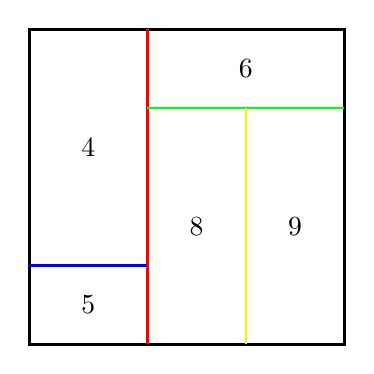
\begin{tikzpicture}  
      \draw[very thick] (2,-2) rectangle (6,2);
  
      \draw[thick, red] (3.5,-2) -- (3.5,2);
      \draw[thick, blue] (2,-1) -- (3.5,-1);
      \draw[thick, green] (6,1) -- (3.5,1);
      \draw[thick, yellow] (4.75,1) -- (4.75,-2);

      \node at (2.75,.5) {4};
      \node at (2.75,-1.5) {5};

      \node at (4.75,1.5) {6};
      \node at (4.125,-.5) {8};
      \node at (5.375,-.5) {9};


    \end{tikzpicture}
    \end{center}
    \end{minipage}&
    \begin{minipage}{.5\textwidth}
      \begin{center}
      \textbf{Baum}
      \end{center}
    \begin{center}
    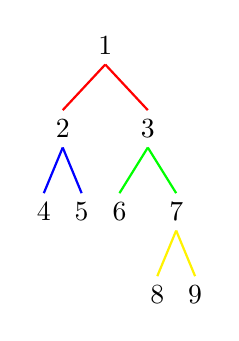
\begin{tikzpicture}
      \Tree[ .1 \edge[draw=red,thick];[ .2 \edge[draw=blue,thick];4 \edge[draw=blue,thick];5 ] \edge[draw=red,thick];[ .3 \edge[draw=green,thick];6 \edge[draw=green,thick];[ .7 \edge[draw=yellow,thick];8 \edge[draw=yellow,thick]; 9 ] ] ]
    \end{tikzpicture}
    \end{center}
    \end{minipage}
  \end{tabular}
\caption{Space Partitioning mit $k$-d-Baum}
\label{04spdgkdtree}
\end{figure}

Ein ähnlicher Algorithmus zur Unterteilung rechteckiger zweidimensionaler Flächen in Partitionen verwendet Quadtrees. Hier wird eine Fläche in jedem Schritt in vier Partitionen unterteilt. Damit hat jeder Knoten im Baum entweder keine Kinder oder genau vier Kinder. Bei der Partitionierung einer Fläche kann für jede Achse ein Punkt zufällig gewählt werden, an dem die Fläche partitioniert wird. Alternativ kann eine Fläche auch in vier gleich große Partitionen unterteilt werden. Letztere Methode kann genutzt werden, um einen im Vergleich zu den zufälligen Methoden gleichmäßigeren Dungeon zu generieren. Eine weitere Möglichkeit zur Erstellung der Partitionen an einem Knoten ist es die Fläche zunächst in vier gleich große Partitionen zu unterteilen, den Algorithmus jedoch nur auf einer, zwei oder drei der Partitionen rekursiv aufzurufen. Die restlichen Partitionen werden in diesem Fall direkt zu Blättern im Baum. Als Abbruchkriterien können die gleichen, wie bei $k$-d-Bäumen verwendet werden. Abbildung \ref{04spdgquadtree} zeigt die Partitionierung einer quadratischen Fläche mit einem Quadtree, wobei in jedem Schritt in vier gleich große Partitionen unterteilt wird.

Für beide Algorithmen lassen sich weitere Methoden zur Partitionierung der Ausgangsfläche, sowie weitere Abbruchkriterien finden. Weiterhin existieren Verallgemeinerungen bzw. Methoden für dreidimensionale Räume, wie z.B. Octrees. 

\begin{figure}[h]
    \centering        
    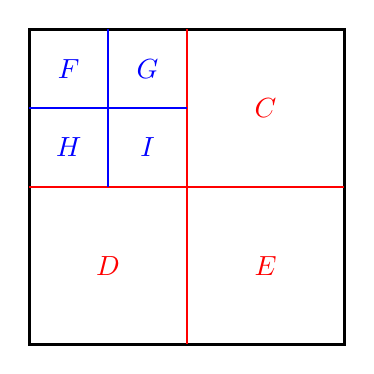
\begin{tikzpicture}
      \draw[very thick] (-2,2) rectangle (2,-2);
      \draw[thick, red] (0,2) -- (0,-2);
      \draw[thick, red] (-2,0) -- (2,0);
      \draw[thick, blue] (-1,2) -- (-1,0);
      \draw[thick, blue] (-2,1) -- (0,1);
      \node at (1,1) {$\textcolor{red}C$};
      \node at (-1,-1) {$\textcolor{red}D$};
      \node at (1,-1) {$\textcolor{red}E$};
      \node at (-1.5,1.5) {$\textcolor{blue}F$};
      \node at (-.5,1.5) {$\textcolor{blue}G$};
      \node at (-1.5,.5) {$\textcolor{blue}H$};
      \node at (-.5,.5) {$\textcolor{blue}I$};
    \end{tikzpicture}\hspace{1.5cm}
    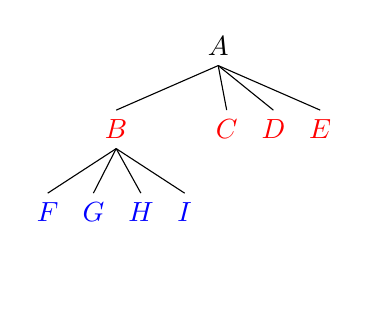
\begin{tikzpicture}
      \Tree [.$A$ [.$\textcolor{red}B$ $\textcolor{blue}F$ $\textcolor{blue}G$ $\textcolor{blue}H$ $\textcolor{blue}I$ ] $\textcolor{red}C$ $\textcolor{red}D$ $\textcolor{red}E$ ]
      \node at (0,-3) {};
    \end{tikzpicture}          
    \caption{Space Partitioning mit Quadtrees}  
    \label{04spdgquadtree}      
\end{figure}

\subsection{Platzierung der Räume und Korridore}
Ausgehend von einer in einer mittels Space Partitioning erstellten Baumstruktur vorliegenden Partitionierung einer rechteckigen Fläche können nun Räume in den Partitionen platziert werden. Da die Partitionen zunächst direkt aneinander anliegen, werden die Räume mit einem durch Parameter beschränkten, zufällig gewählten Abstand zu der linken, rechten, oberen und unteren Begrenzung platziert. Nach der Platzierung der Räume wird der Baum traversiert, um Räume durch Korridore miteinander zu verbinden. Dazu wird in jedem Knoten ein Korridor generiert, der zwei Räume in den Partitionen der Teilbäume der Kinder miteinander verbindet. Der Korridor verläuft dabei durch eine in dem Knoten gespeicherte Unterteilungsebene, wodurch sichergestellt wird, dass Korridore sich nicht überschneiden. Ein Beispiel für einen prozedural generierten Dungeon mit zugehörigem $k$-d-Baum ist in Abbildung \ref{04spdgdungeon} gegeben. Der blau markierte Korridor wurde beispielsweise im Knoten $0$ platziert.
\begin{figure}[h]
    \centering
    \begin{tabular}{cc}
        \begin{minipage}{.4\textwidth}
            \includegraphics[width = 0.8\textwidth]{resources/img/sp_ex_l3.jpeg}
        \end{minipage}
            &\begin{minipage}{.4\textwidth}
                \includegraphics[width = 0.8\textwidth]{resources/img/sp_ex_tree.png}
            \end{minipage}
    \end{tabular}
\caption{Prozedural generierter Dungeon mit $k$-d-Baum}
\label{04spdgdungeon}
\end{figure}

	
	\chapter{Technische Umsetzung}
\label{Technische_Umsetzung}

\section{Creature Generation}
% Einleitung
%   - Ziel: Rechtfertigung technischer design entscheidungen, plus überblick über den Code
%   - Creature Generator als Unity Package
%   - Erläutere Aufbau des Kapitels
%       - Der Pipeline folgend, von der Bone Definition, bis zur Creature Generator Klasse
% Settings als ScriptableObjects
%   Creature Parameters
%       - Funktion als zentrales Einstellungsobjekt des Generators
%       - Tabelle mit momentanen Einstellungen
%   Creature Generator Settings
% Bone Definition
%   - Existenzgrund: Generische Datenstruktur für alle möglichen Generatoren
%   - Erläuterung der Datenstruktur
%   - Anatomische Koordinatensysteme
%       - Verweis auf Fachliches Vorgehen für Details
%       - Technischer Grund: Annahmen über Koordinatensysteme werden nicht über Generator grenzen getragen
% Generator Klassen
%   - Instanziieren der Creature Parameters um Knochenlängen an AI zu liefern
%   - Zusammenstecken der Bone Definitions
% Skeleton Definition
%   - 
% Joint Tables und Density Tables
% Skeleton Assembler
%   - Erzeugt Unity Gameobjects aus der Skeleton Definition
% Mesh Generator

Das folgende Kapitel ist eine Tour durch den PG649 Creature Generator und wird die wichtigsten Datenstrukturen und Klassen erläutern.
Ziel der Tour ist es sowohl eine Hilfe beim Lesen des Quellcodes zu sein, als auch Design-Entscheidungen und Trade-Offs zu erläutern.

\subsection{Unity Package}
Der Generator wird als unabhängiges Unity Package entwickelt.
So kann der Generator einfach in KI-Lernumgebungen und das spätere Spiel eingebunden werden und es wird eine saubere API für den Generator ermutigt.

Die Dateistruktur des Generators unterscheidet sich damit von einem typischen Unity Projekt. Statt im \texttt{Assets}-Ordner, liegen alle hier erläuterten Klassen in \linebreak\texttt{Packages/com.pg649.creaturegenerator/Runtime}.
Der \texttt{Assets}-Ordner enthält lediglich Debug-Skripte, die nicht exportiert werden sollen.

\subsection{Konfiguration}
Die Klassen \texttt{Creature\-Generator\-Settings} und \texttt{Parametric\-Creature\-Settings} enthalten alle Konfigurationsmöglichkeiten für den Generator.
Sie sind der Hauptweg mit dem Nutzer mit dem Generator interagieren und bilden somit den Anfang der Tour. 

Die Klasse \texttt{CreatureGeneratorSettings} enthält Einstellungen, die das Verhalten des Generators und der generierten Kreaturen bestimmen.
Dazu gehören Einstellungen die zum Beispiel das generieren eines Meshes für die Kreatur abschalten, Einstellungen für das physikalische Verhalten der Kreature, sowie Einstellungen für Debug-Optionen.
Die individuellen Einstellungen sind in der Klasse selbst dokumentiert und werden hier nicht einzeln aufgeführt.

Die Klasse \texttt{ParametricCreatureSettings} enthält Einstellungen, die das Aussehen der generierten Kreaturen bestimmen.
Die Einstellungen definieren Intervalle für die erlaubte Länge, Dicke, und ggbf. Anzahl für Knochen bestimmter Kategorien.
Wieder sind die individuellen Einstellungen in der Klasse selbst dokumentiert.

Beide Konfigurationsklassen sind sogenannte \texttt{ScriptableObjects}.
Sie können von Unity serialisiert und als Assets gespeichert werden.
So können für das spätere Spiel Einstellungen für verschiedene Kreaturen genau so mit exportiert werden wie beispielsweise Shader.
Außerdem ist es möglich die Einstellungen mittels \texttt{git} zu versionieren.

\subsection{Bone Definition}
Eine der ersten Datenstrukturen, die von dem Generator erzeugt werden, ist ein Baum von \texttt{BoneDefinition}s.
Dieser Baum bildet die abstrakteste Darstellung eines Skeletts und dient als generisches Ziel für die Generatoren der verschiedenen Kreaturen-Typen.
Jede \texttt{BoneDefinition} enthält die Details eines Knochens, d.h. um was für einen Knochen es sich handelt (Arm, Bein, etc.), die Länge und Dicke des Knochens, die Ausrichtung seines lokalen Koordinatensystems, und Informationen dazu, wie der Knochen für das finale Skelett an seinem Eltern-Knochen angebracht werden soll.

Letztere Informationen werden \texttt{AttachmentHint} genannt und erlauben es Knochen relativ zur Größe des Elternknochens zu positionieren, sie um einen absoluten Vektor zu verschieben, die ventrale Achse des Koordinatensystems auszurichten, und zuletzt den Knochen in eine gewünschte Ausgangspose zu rotieren.
So können humanoide Kreaturen beispielsweise in die typische T-Pose gebracht werden.

Es gibt drei Gründe das lokale Koordinatensystem eines jeden Knochens explizit anzugeben:
\begin{itemize}
    \item Quellcode außerhalb der, später beschriebenen, paramatrischen Generatoren ist nicht durchsetzt mit Konventionen und Annahmen über Koordinatensysteme; Statdessen sind die gewählten Koordinatensysteme explizit.
    \item es erlaubt die Wahl von semantisch bedeutungsvollen Koordinatenachsen (Proximal, Ventral, Lateral)
    \item es erlaubt unterschiedlichen parametrischen Generatoren eigene Konventionen für ihre Koordinatensysteme zu wählen.
\end{itemize}

\subsection{Parametrische Generatoren}
Parametrische Generatoren haben die Aufgabe anhand der \texttt{Parametric\-Creature\-Settings} \texttt{Bone\-Definition}-Bäume zu generieren.
Das Package enthält momentan Generatoren für zwei verschiedene Typen von Kreaturen: \texttt{BipedGenerator} und \texttt{QuadrupedGenerator}.
Einstiegspunkte in die Generatoren sind jeweils die \texttt{BuildCreature} Methoden.

Beide Generatoren erzeugen zunächst aus den Intervallen in den \texttt{Parametric\-Creature\-Settings} zufällig tatsächliche Längen, Dicken, and Anzahlen in Form einer \texttt{Biped\-Settings\-Instance} bzw. \texttt{Quadruped\-Settings\-Instance}.
Die generierte Einstellungs\--Instanz ist später Teil der Metadaten die zusammen mit der Kreatur zur Verfügung gestellt werden und wird während des Lern-Prozesses genutzt.
Zu diesem Zweck implementieren sie das \texttt{ISettings\-Instance}-Interface.
Die Werte anfangs zu generieren erleichtert es außerdem die Symmetrie der Kreatur sicherzustellen.

Um die Kreaturen später trainieren zu können, müssen sie mehrfach generierbar sein.
Beide Generatoren akzeptieren deshalb einen Seed für den Zufallsgenerator. Dabei ist zu beachten, dass der selbe Seed in der selben Version des Packages die selbe Kreatur erzeugen wird. Der Aufwand die Stabilitäts-Garantie auch über Package Versionen hinweg zu garantieren, wurde für nicht nötig gehalten und wurde nicht betrieben.

Nachdem die Parameter der Knochen finalisiert wurden, konstruieren beide Generatoren einen Baum aus \texttt{BoneDefinition}s.
\todo{Explain tree structure if not done in chapter 5}

\subsection{Skeleton Definition}
Die Ausgabe der Parametrischen-Generatoren ist eine \texttt{Skeleton\-Definition}, bestehend aus dem \texttt{Bone\-Definition}-Baum, der Einstellungs-Instanz, und einem \texttt{Limit\-Table}.
Die \texttt{LimitTable}-Klasse ist dabei eine Tabelle, die festhält um welche Koordinatenachsen und wie weit sich jeder Knochen rotieren darf.

Die \texttt{Skeleton\-Definition} dient dann im nächsten Schritt als Eingabe für den \texttt{Skeleton\-Assembler}.

\subsection{Skeleton Assembler}
Der \texttt{Skeleton\-Assembler} baut aus der \texttt{Skeleton\-Definition} einen Baum aus Unity \texttt{Game\-Object}s, der dann in Szenen als Ragdoll verwendet werden kann. Einstiegspunkt dafür ist die Methode \texttt{Assemble}.

In einem ersten Durchgang wird für jede \texttt{Bone\-Definition} des Baumes ein \texttt{Game\-Object} erstellt. Jedes dieser \texttt{GameObject}s wird mit mehreren Komponenten ausgestattet:
\begin{itemize}
    \item ein \texttt{Rigidbody}, damit physikalische Kräfte auf den Knochen wirken können
    \item ein \texttt{Collider}, damit der Knochen mit anderen Objekten kollidieren kann. Die Form des \texttt{Colliders} hängt vom Typen des Knochen ab.
    \item ein \texttt{Bone}, der Metadaten, wie z.B. Länge oder Kategorie des Knochens, enthält, aber auch die Farbe des Knochens für die spätere Darstellung im Spiel
\end{itemize}
Die Farbe des Knochens wird zufällig im HSV Farbraum generiert und dann in das in der Computergrafik übliche RGB Format konvertiert.
Der HSV Farbraum erleichtert es zufällig Farben in bestimmten Farbtönen und Helligkeiten zu generieren, in unserem Fall zombieartige Grüntöne.

Die Masseberechnung für den Rigidbody verdient ebenfalls besonderes Augenmerk.
Der \texttt{SkeletonAssembler} berechnet die Masse des \texttt{Rigidbodies} grundsätzlich aus dem Volumen des an dem ihm angebrachten \texttt{Colliders} und der Dichte des Knochens, die der \texttt{SkeletonAssembler} einem \texttt{DensityTable} entnimmt.
In der Praxis führen zu große Unterschiede in der Masse von zwei durch einen \texttt{ConfigurableJoint} verbundenen \texttt{Rigidbodies} zu numerischer Instabilität in der Physiksimulation, weshalb der \texttt{SkeletonAssembler} optional in jedem \texttt{Rigidbody} die selbe fixe Masse setzen kann.

Der Wurzel-Knochen wird zusätzlich mit einer \texttt{Skeleton}-Komponente ausgestattet, die weitere Metadaten über das Skelett als ganzes enthält und einfaches iterieren über alle Knochen erlaubt.

Die Nicht-Wurzel Knochen werden entsprechend ihres \texttt{Attachment\-Hint}s positioniert.
Lediglich die Rotation in die Ausgangspose wird noch nicht angewandt, da dies die Ausrichtung der ventralen Achse aller Knoten unterhalb des momentanen Knoten beeinflussen würde.

Optional wird an dieser Stelle ein weiteres \texttt{Game\-Object} unter jeden Knoten gehangen, welches ein Mesh enthält, dass den \texttt{Collider} des Knochens visualisiert.

In einem weiteren Durchgang wird das Skelett zunächst in seine Ausgangspose rotiert.
Danach werden Eltern-Kind Paare von Knochen mittels Unitys \texttt{Configurable\-Joint}-Komponente verbunden.
Die Reihenfolge ist hier essentiell, da die Joints die Position der Knochen zum Zeitpunkt der Erstellung der Joints als Ruheposition ansehen.

Die \texttt{Configurable\-Joint}s erlauben das setzen einer Ziel-Position und Ziel-Rotation und errechnen dann selbstständig die nötigen Kräfte, die auf ihren verbundenen Körper wirken müssen, um diese zu erreichen.
Die Machine-Learning Verfahren produzieren Ziel-Rotationen für jeden Joint.
Die Joints sind damit Herzstück des Bewegungssystems und ihre Konfiguration wird daher später näher erläutert.

Zuletzt wird noch der Wurzel-Knochen markiert und die von dem parametrischen Generator erzeugte Einstellungs-Instanz in der \texttt{Skeleton}-Komponente hinterlegt.

\subsubsection{Configurable Joints}
Die lineare Bewegung der Joints wird für fast alle Knochen vollständig gesperrt.
Dazu werden die \texttt{xMotion}, \texttt{yMotion}, \texttt{zMotion} Felder auf \texttt{Locked} gesetzt.
Die Joints halten nun, soweit physikalisch möglich, ihre Position relativ zum Eltern-Knochen.
Lediglich für Knochen die im \texttt{BoneTree} direkt unterhalb eines Hüft- oder Bein-Knochens liegen wird eine lineare Bewegung entlang der der z-Achse (proximalen Achse) erlaubt und eine entsprechende Feder konfiguriert, um die zuvor beschriebenen Stoßdämpfer zu modellieren. 

Die Rotation der Joint wird entsprechend der \texttt{Limit\-Table} eingeschränkt.
Die \texttt{angular\-XMotion}, \texttt{angular\-YMotion}, \texttt{angular\-ZMotion} Felder werden entsprechend auf \texttt{Locked} oder \texttt{Limited} gesetzt, und die dazugehörigen \texttt{angularLimits} werden ausgefüllt.
Dabei gibt es zwei Dinge zu beachten.

Zum einen erlauben die Joints nur für die x-Achse die Angabe eines minimalen und maximalen Winkels, Rotationen um die y- und z-Achse können nur symmetrisch eingeschränkt werden.
Allerdings haben die Joints ein eigenes Koordinatensystem separat von dem des Knochens.
Der \texttt{Limit\-Table} enthält deshalb gegebenenfalls außerdem Informationen darüber welche Koordinatenachse des Knochens als x-Achse des Joints fungieren soll.

Zum anderen müssen Knochen behandelt werden, die zueinander gespiegelt sind. So muss zum Beispiel der eine Arm eines Zweibeiners im Uhrzeigersinn rotieren, um nach vorne bewegt zu werden, der andere aber gegen den Uhrzeigersinn. Die \texttt{Bone}-Komponenten enthalten deshalb das Feld \texttt{Mirrored}, was angibt ob der Knochen gespiegelt ist. Ist der Knochen gespiegelt, so werden die Koordinatenachsen des Joint-Koordinatensystems mit \(-1\) multipliziert. So genügt ein einzelner Eintrag im \texttt{Limit\-Table} für beide Versionen des Knochens.

Der \texttt{projectionMode} des Joints wird auf \texttt{Postion\-And\-Rotation} gestellt, um den Joint zu zwingen die gesetzten Rotations-Limits einzuhalten und für Debug-Zwecke wird der \texttt{slerpDrive} initialisiert, damit der Joint Kraft aufwenden kann.

\subsection{Mesh Generator}
Das Mesh der Kreatur wird mit Hilfe der Klasse \texttt{Metaball} erzeugt Einem Metaball-Objekt können einzelne Körper über die Methode \texttt{AddBall} hinzugefügt werden. Diese werden durch die Klasse \texttt{Ball} realisiert. Um andere Körper als Kugeln erstellen zu können, muss eine Klasse erstellt werden, die von \texttt{Ball} erbt und die Distanzfunktion anpasst, wie wir es für die \texttt{Capsule} getan haben. Die Definitionen verschiedener Falloff-Funktionen sind ebenfalls in der Ball-Klasse implementiert. Die jeweils verwendete Funktion wird als Enumeration über einen Parameter übergeben.\\
Die Klasse \texttt{Metaball} enthält außerdem eine statische Methode \texttt{BuildFromSkeleton}, die das Mesh für ein gesamtes Skelett erzeugt. Dabei wird für jeden Knochen eine korrekt skalierte Metakapsel an der richtigen Position erstellt.\\
Aus der daraus resultierenden impliziten Definition der Oberfläche wird anschließend das diskrete Mesh generiert, dies ist durch die Klasse \texttt{MeshGenerator} und die darin enthaltene Methode \texttt{Generate} realisiert. Über das Klassenattribut \texttt{gridResolution} lässt sich die Auflösung des zur Abtastung verwendeten Gitters einstellen. Unsere Implementierung des Marching Cubes Algorithmus basiert auf einem existierenden Projekt des GitHub-Users Scrawk \cite{MarchingCubesImplementation} .

\subsection{Creature Generator}
Der oben beschriebene Ablauf des Creature-Generators ist implementiert in der Klasse \texttt{Creature\-Generator}, die zugleich das öffentliche Interface des Generators ist. Die Methoden \texttt{Parametric\-Biped} und \texttt{Parametric\-Quadruped} erstellen jeweils die passende \texttt{Skeleton\-Definition} und übergeben sie an die Methode \texttt{Parametric}, die daraus die vollständige Kreatur generiert.


\section{Creature Animation}
% !TeX spellcheck = de_DE

\subsection{Trainingsumgebung}
Im Folgenden soll der Aufbau der Trainingsumgebung beschrieben werden, welche es erlaubt verschiedenste Kreaturen ohne große Anpassungen zu trainieren. Die  Umgebung ist dabei aus den folgenden Klassen aufgebaut:

\begin{itemize}
	\item \texttt{DynamicEnviormentGenerator}
	\begin{itemize}
		\item \texttt{TerrainGenerator} %Todo change when replaced by package
		\item Verschiedenen Konfigurationsdateien
		\item \texttt{DebugScript}
	\end{itemize}
	\item allen anderen modifizierten ML-Agents Skripten
\end{itemize} 

In diesen Abschnitt wird nur auf den Aufbaue des \texttt{DynamicEnviormentGenerator} sowie dessen Hilfsklassen und nicht auf die ML-Agent-Skripte eingegangen. Die Hilfsklassen sind der \texttt{TerrainGenerator}, \texttt{GenericConfig} und dessen Implementierungen sowie das \texttt{DebugScript}. Erstere ist verantwortlich für die Generierung des Terrains, die Config-Dateien laden dynamisch die Einstellungen aus einer Datei und das letzte Skript beinhaltet hilfreiche Debug-Einstellungen. Die grundsätzliche Idee der Trainingsumgebung stammt von dem ML-Agents-Walker. Da an diesem keine Versuche mit Unterschiedlichen Umgebungen und Kreaturen durchgeführt wurden, ist der Aufbau des Projekts nicht dynamisch genug. 

\subsubsection{Dynamic Enviorment Generator}
Zur dynamischen Umsetzung der Trainingsarena werden alle Objekte zur Laufzeit erstellt. Die Generierung der Arena läuft dann wie folgt ab:
\begin{enumerate}
	\item Erstellen von $n$ Arenen, wobei $n$ eine zu setzende Variable ist. 
	\item Füge ein Ziel für die Kreatur in die Arena ein
	\item Generiere die Kreatur
\end{enumerate}

Die einzelnen (Teil)-Arenen bestehen aus einem Container-Objekt unter dem ein Terrain und vier Wall-Prefabs angeordnet sind. Diese Prefabs und weitere Elemente wie Texturen werden dynamisch aus einem Ressourcen-Ordner geladen, damit möglichst wenige zusätzliche Konfigurationen den Editor verkomplizieren. Das Terrain wird mit leeren Terraindaten vorinitialisiert und später befüllt. Hierbei kann die Position des Container-Objects in der Szenen wie folgt berechnet werden:
\begin{align}
	\begin{pmatrix}
	\lceil \frac{\text{Anzahl der Arenen}}{\sqrt{\text{Anzahl der Arenen}}} \rceil \\
	0 \\
	\text{Anzahl der Arenen} \mod \sqrt{\text{Anzahl der Arenen}} \\
	\end{pmatrix}
	 = 	\begin{pmatrix}
	 x  \\
	 y \\
	 z  \\
	 \end{pmatrix}
\end{align}
Alle anderen Objektpositionen müssen danach neu im lokalen Koordinatensystem gesetzt werden. Da die Unity-Standard-Texturen sehr hell sind sind, werden die Texturen bei der Initialisierung mit ML-Agents-Texturen, welche dunkler sind, getauscht. An das Terrain werden zuletzt Collider und ein \texttt{TerrainGenerator}-Skript angefügt. 

In Schritt 2. der Arenagenerierung muss beachtet werden, dass nach dem Erstellen des Zielobjekts das \texttt{WalkTargetScript} hinzugefügt wird. Am Ende des Erstellungsprozesses wird der Walker erstellt. Hierzu wird ein von den Creature-Generator-Team bereitgestelltes Paket\footnote{https://github.com/PG649-3D-RPG/Creature-Generation} benutzt. Das Paket stellt ein Klasse bereit, welche mit zwei Skript-Objekte konfiguriert wird. Zusätzlich wird ein seed übergeben, welcher reproduzierbare Kreaturen erlaubt. Die erstelle Kreatur muss danach mit den entsprechenden ML-Agent-Skripten versehen werden. Hierzu wird ein \texttt{WalkerAgent} Objekt als String übergeben. Dies ermöglicht es, mehrere unterschiedliche Agent-Skripte durch eine Änderung im Editor zu setzen. Somit können Reward-Funktion und Observation für zwei unterschiedliche Trainingsversuche getrennt, in eigenen Dateien, entwickelt werden.
\begin{figure}
	\centering
	\includegraphics[width=0.7\linewidth]{example-image-a}
	\caption[Konfigurationsmöglichkeiten des \texttt{DynamicEnviormentGenerator}]{Konfigurationsmöglichkeiten des \texttt{DynamicEnviormentGenerator} im Unity-Editor.} %TODO setz pictures
	\label{bspDEGOptionen}
\end{figure}

\begin{figure}
	\centering
	\includegraphics[width=0.7\linewidth]{example-image-a}
	\caption[Beispiel der generierten Trainingsumgebung]{Ein Beispiel der generierten Trainingsumgebung mit mehreren Arenen.} %TODO setz pictures
	\label{bspArena}
\end{figure}

\subsubsection{TerrainGenerator}
Da ein typisches Spieleterrain im Gegensatz zum ML-Agents-Walker-Terrain nicht flach ist, wurde ein neues Objekt erstellt, welches sowohl die Generierung von Hindernissen, als auch eines unebenen Bodens erlaubt. Um ein möglichst natürlich erscheinendes Terrain zu erzeugen wird ein Perlin-Noise verwendet. Dieses spiegelt jeweils die Höhe des Terrains an einen spezifischen Punkt wider. Im späteren Projektverlauf wurde dieses Skript durch den Terraingenerator des dazugehörigen Teams ersetzt.

\subsubsection{Konfigurationsobjekte}
Da sich die statische Konfiguration des ML-Agents-Walker als problematisch erwies, wurde die Konfiguration über die Laufzeit des Projekts dynamischer gestaltet. Zuerst wurden alle Konfigurationen im \texttt{DynamicEnviormentGenerator} gespeichert. Was unübersichtlich war und zu ständigen neubauen des Projektes führte. Deshalb wurde eine \texttt{GenericConfig} Klasse eingeführt, welche die im Editor eingestellten Optionen für die einzelnen Teilbereiche Terrain, Arena und ML-Agent in Json-Format in den Streaming-Asset-Ordner speichert. Da dieser Ordner beim bauen des Projekts in das fertige Spiel übertragen wird, sind diese Konfigurationen automatisiert dort vorhanden. 

Im Fall, dass das Spiel ohne Editor gestartet wird, was meist beim Training der Fall ist, lädt das generische Objekt aus den Json-Dateien die Einstellungen und ersetzt die Editorkonfiguration damit. Hierdurch ist ein ändern der Konfiguration des Spiels ohne neu-erstellen der Binärdateien ermöglicht. Diese Konfigurationsart fügt Abhängigkeiten zu dem Unity eigenen JsonUtility\footnote{https://docs.unity3d.com/ScriptReference/JsonUtility.html} hinzu.

\subsection{WalkerAgent/blabla}
Jan mach mal! Irgendwo auch Generalisierung
\begin{itemize}
	\item UML von den Klassen
	\item WalkerAgent/JointDriveController/TargetController
	\item Reward Funktion
\end{itemize}

\subsection{LiDO3}
% Nils
Wie bereits erwähnt, werden die Berechnungen jeweils auf den HPC der TU Dortmund ausgeführt. Um auf LiDO3 zu arbeiten wird mit Hilfe eines Gatewayservers auf das Cluster zugegriffen. Der Zugriff ist ausschließlich über das TU Dortmund Netzwerk möglich. Über den Gatewayserver kann ein Zugriff auf die Rechenressourcen direkt über die Shell oder über Skripte angefordert werden. Da die Shell-Methode einen dauerhaften Login erfordern würde, wird mit Skripten gearbeitet. Diese bestehen aus Konfigurationen für LiDO3 und den eigentlich Programmteil, welcher ausgeführt werden soll. LiDO3 nutzt als Jobmanager Slurm, weshalb die Skripte die Slurm-Syntax nutzen. Eine ausführliche Beschreibung die LiDO3 Konfiguration findet sich im Benutzerhandbuch\cite{lido};

% TODO hier Skript richtig einfügen
\label{prog:lidoSkript}
\begin{verbatim}
#!/bin/bash -l
#SBATCH -C cgpu01
#SBATCH -c 20
#SBATCH --mem=40G
#SBATCH --gres=gpu:2
#SBATCH --partition=long
#SBATCH --time=48:00:00
#SBATCH --job-name=pg_k40
#SBATCH --output=/work/USER/log/log_%A.log
#SBATCH --signal=B:SIGQUIT@120
#SBATCH --mail-user=OUR_MAIL@tu-dortmund.de
#SBATCH --mail-type=ALL
#-------------------------------------

GAME_NAME="GAME_NAME"
GAME_PATH="/work/USER/games/$GAME_NAME"


module purge
module load nvidia/cuda/11.1.1

source /work/USER/anaconda3/bin/activate
conda activate /work/mmarplei/grudelpg649/k40_env

chmod -R 771 $GAME_PATH
cd $GAME_PATH

srun mlagents-learn /work/smnidunk/games/config/Walker.yaml --run-id=$GAME_NAME --env=t.x86_64 --num-envs=6 --no-graphics

\end{verbatim}

In dem Beispielskript \ref{prog:lidoSkript} sind Anweisungen an die LiDO-Umgebung jeweils mit einem Kommentarzeichen gefolgt von \emph{SBATCH} gekennzeichnet. Die Konfiguration wird so gewählt, dass eine maximale Laufzeit mit exklusiven Ressourcenrechten auf den Rechenknoten besteht. Zusätzlich muss sichergestellt werden, dass eine Grafikkarte zur Verfügung steht. Diese stehen auf den \emph{cgpu01}-Rechenknoten mit jeweils 20 CPU-Kernen und 48 Gigabyte RAM zur Verfügung. Die maximale Laufzeit des Prozesses ist bei den GPU-Knoten auf \emph{long} begrenzt, was 48 Stunden entspricht. Es wird jeweils ein Log mitgeschrieben, aus dem der Trainingsfortschritt gelesen werden kann und bei besonderen Ereignissen eine Mail geschickt, um sofort benachrichtigt zu werden, falls der Job fertig ist oder fehlschlägt.

\subsubsection{Kompatibilitätsprobleme}
Um das beschriebene Skript auszuführen, muss auf LiDO3 eine ML-Agents-Umgebung installiert werden. Dabei handelt es sich um ein Python Umgebung, mit PyTorch und CUDA. In dem Slurm-Skript \ref{prog:lidoUmgebung} ist die Einrichtung einer funktionierenden Umgebung dargestellt. 

\label{prog:lidoUmgebung}
% TODO hier Skript richtig einfügen
\begin{verbatim}
// LIDO UMGEBUNGSVARIABLEN
module purge
module load nvidia/cuda/11.1.1

source <anaconda3-path>/bin/activate
conda activate <env_to_install>
conda install torchvision torchaudio cudatoolkit=11.1 -c pytorch
python -m pip install mlagents==0.29.0 --force-reinstall
python -m pip install /work/mmarplei/grudelpg649/torch-1.10.0a0+git3c15822-cp39-cp39-linux_x86_64.whl --no-deps --force-reinstall 
\end{verbatim}

Für die Python-Installation wurde auf Anaconda\footnote{https://www.anaconda.com/} zurückgegriffen. Die installierte Anaconda-Arbeitsumgebung kann für die folgenden Schritte genutzt werden, indem die Slurm-Skripte diese am Anfang laden. CUDA kann als Kernelmodul in verschiedenen Versionen geladen werden oder per Anaconda installiert werden.

Problematisch ist die Installation von PyTorch, da ab Version 1.5 die Installationsbinärdateien keine Unterstützung für die von LiDO3 genutzten NVIDIA Tesla K40 Grafikarten bietet. Es besteht die Möglichkeit PyTorch zu bauen um die Unterstürzung zu erhalten. Dies musste für unsere Arbeitsumgebung nicht gemacht werden, da die PG-Betreuer ein Paket mit einer für LiDO funktionierenden PyTorch-Version von einer vorherigen PG zur Verfügung stellen konnten. Wie in \ref{prog:lidoUmgebung} dargestellt müssen zuerst die Abhängigkeiten von PyTorch, dann ML-Agents und zuletzt die spezielle PyTorch Version installiert werden, da sonst die Abhängigkeiten Probleme bereiten.



	
	\chapter{Evaluation}
\label{chap:evaluation}
In diesem Kapitel wird die Trainingsqualität der generierten Kreaturen evaluiert. 

\section{Einschränkungen der Evaluation}

\subsection{Auswahl der Kreaturen}
Die Evaluation wird aufgrund der limitierten Rechenressourcen auf jeweils eine Vierbeiner Kreatur und eine Zweibeiner Kreatur beschränkt. Abbildung \ref{fig:4B_creature_settings} zeigt die Parameter zur Generierung der Vierbeiner Kreatur. Abbildung \ref{fig:2B_creature_settings} zeigt die Parameter zur Generierung der Zweibeiner Kreatur.

\begin{figure}[ht]
    \centering
    \includegraphics[width=0.5\linewidth]{example-image-a}
    \caption{4B Parameter}\label{fig:4B_creature_settings}
\end{figure}

\begin{figure}[ht]
    \centering
    \includegraphics[width=0.5\linewidth]{example-image-a}
    \caption{2B Parameter}\label{fig:2B_creature_settings}
\end{figure}

\subsection{Konfiguration der Trainingsdurchläufe}
Die Erfahrung während der Entwicklungsphase der Projektgruppe hat gezeigt, dass die verwendete PPO Implementierung weitestgehend robust gegenüber der verwendeten Hyperparameter ist, solange eine ausreichend große Batchgröße verwendet wird. Aufgrund der limitierten Rechenressourcen wurde deswegen auf eine Hyperparameteroptimierung verzichtet. Abbildung \ref{fig:evaluation_config} zeigt die für die Evaluation verwendete neroRL Konfigurationsdatei. 
Für die Trainingsdurchläufe werden Unity Builds mit 16 Agenten verwendet, die auf 8 parallelen Workern ausgeführt werden. Dementsprechend werden die Daten parallel von 128 Agenten gesammelt. Jeder Agent führt bei jeder fünften Aktualisierung der Physikengine eine Aktion aus. Für das Training wird eine Batchgröße von 102400 verwendet, somit entsprechen 10 Updates etwa 1 Mio Schritten in der Umgebung.
Die in Abschnitt \ref{} beschriebenen Reward-Funktionen für das Aufstehen und Laufen werden jeweils zwei Mal für die Vierbeiner Kreatur und zwei Mal für die Zweibeiner Kreatur trainiert. Dabei werden alle 100 Updates die Policies zwischengespeichert und zum Sammeln der Evaluationsdaten verwendet. Für die Evaluation werden mit den gespeicherten Policies jeweils 128 zufällige Episoden ausgeführt und dabei Reward und Episodenlänge gesammelt.

\begin{figure}[ht]
    \centering
    \includegraphics[width=0.5\linewidth]{example-image-a}
    \caption{neroRL Konfigurationsdatei für die Evaluation}\label{fig:evaluation_config}
\end{figure}


\section{Ergebnisse}
In diesem Abschnitt werden die Ergebnisse der Trainingsdurchläufe für die Vierbeiner und Zweibeiner Kreaturen beschrieben. Zunächst werden Daten bezüglich des Rewards und der Länge der Trainingsepisoden analysiert. Anschließend wird die Qualität der Trainingsergebnisse bei der visuellen Evaluation in Unity beschrieben.

\subsection{Vierbeiner Kreatur}

\subsubsection{Laufen}
Die Entwicklung des Rewards beim Trainieren des Laufens der Vierbeiner Kreatur ist in Abbildung \ref{fig:Walking4B_Reward} abgebildet. Der Reward steigt in den ersten 1000 Updates deutlich an und erreicht ein Maximum von 14000. Danach fällt der Reward langsam ab auf ca. 7000-1000, ein Policy Collapse tritt nicht ein. 

\begin{figure}[ht]
    \centering
    \includegraphics[width=0.5\linewidth]{resources/img/results/Walking4B_Reward.png}
    \caption{Walking 4B Reward}\label{fig:Walking4B_Reward}
\end{figure}

Die Episodenlänge der Vierbeiner beim Laufen ist unbeschränkt, eine Episode wird beendet, wenn die Kreatur mit einem Körperteil außer den Füßen den Boden berührt. Da alle 5 Physik-Aktualisierungen der Unity Umgebung eine Aktion des Agenten angefordert wird und die Unity Umgebung mit 120 Aktualisierungen pro Sekunde ausgeführt wird, entspricht eine Länge von 1000 ca. 41.5 Sekunden. Abbildung \ref{fig:Walking4B_Length} zeigt die Entwicklung der Episodenlänge während der Trainingsdurchläufe. Analog zum Reward steigt die durchschnittliche Episodenlänge in den ersten 1000 Updates deutlich an und stagniert danach bzw. fällt langsam ab. Das Maximum wird mit einer Episodenlänge von ca. 6000, umgerechnet ca. 4 Minuten und 9 Sekunden, erreicht.

\begin{figure}[ht]
    \centering
    \includegraphics[width=0.5\linewidth]{resources/img/results/Walking4B_Length.png}
    \caption{Walking 4B Length}\label{fig:Walking4B_Length}
\end{figure}

Die Visuelle Evaluation in Unity zeigt, dass die Vierbeiner Kreatur mit beliebigen Policies ab ca. 500 Updates weitestgehend stabil läuft. Instabilität tritt insbesondere dann auf, wenn die Kreatur mit hoher Geschwindigkeit einen Wegpunkt erreicht und eine große Drehung in Richtung des nächsten Wegpunkts durchführen muss. 

\subsubsection{Aufstehen}
Abbildung \ref{fig:Standup4B_Reward} zeigt die Entwicklung des Rewards während der Updates des Trainingsdurchlaufs. Der Reward steigt in den ersten 250 Updates deutlich von 0 auf ca. 1700. Das Training stagniert für mehrere hundert Updates bei ca. 1700, bevor ein Performance Collapse eintritt, von dem sich die Policy nicht erneut erholt.

\begin{figure}[ht]
    \centering
    \includegraphics[width=0.5\linewidth]{resources/img/results/Standup4B_Reward.png}
    \caption{Standup 4B Reward}\label{fig:Standup4B_Reward}
\end{figure}

Die Episodenlänge für das Aufstehen der Vierbeiner ist auf 1000 Schritte beschränkt und es gibt keine Bedingung, die den Start einer neuen Episode vor Ablauf der Schritte bedingt. Da alle 5 Schritte eine Aktion des Agenten angefordert wird, liegen die in Abbildung \ref{fig:Standup4B_Length} dargestellten Episodenlängen konstant bei 201 Schritten.

\begin{figure}[ht]
    \centering
    \includegraphics[width=0.5\linewidth]{resources/img/results/Standup4B_Length.png}
    \caption{Standup 4B Length}\label{fig:Standup4B_Length}
\end{figure}

Die Visuelle Evaluation in Unity zeigt, dass beliebige Policies aus den Update-Bereichen, in denen der Reward bei ca. 1700 stagniert, in der Lage sind den Vierbeiner erfolgreich aus einer liegenden Startposition aufstehen zu lassen. Die Policies nach dem Performance Collapse führen nur minimal wahrnehmbare Aktionen aus und die Kreatur bleibt unbewegt liegen. 

\subsection{Zweibeiner Kreatur}

\subsubsection{Laufen}
Abbildung \ref{fig:Walking2B_Reward} zeigt die Entwicklung des Rewards beim Trainieren des Laufens der Zweibeiner Kreatur. Der Reward steigt über die ersten ca. 1500 Updates von 0 auf ca. 3000-4000 deutlich an. Danach ist steigt der Reward langsam weiter und schwankt dabei stark. In den Trainingsdurchläufen der Evaluation wurde ein maximaler Reward von ca. 5300 erreicht.

\begin{figure}[ht]
    \centering
    \includegraphics[width=0.5\linewidth]{resources/img/results/Walking2B_Reward.png}
    \caption{Walking 2B Reward}\label{fig:Walking2B_Reward}
\end{figure}

Die Episodenlänge der Zweibeiner beim Laufen ist nicht beschränkt. Eine Episode wird beendet, wenn die Kreatur mit einem Körperteil außer den Füßen den Boden berührt. Die in Abbildung \ref{fig:Walking2B_Length} dargestellte Episodenlänge steigt parallel zum Reward in den ersten 1500 Updates deutlich von 0 auf ca. 1000 und stagniert danach mit Schwankung. Da alle 5 Schritte eine Aktion des Agenten angefordert wird, bedeutet dies ca. 5000 Schritte. Die maximale durchschnittliche Episodenlänge beträgt ca. 2000.

% TODO Ab hier hat Nils dran rumgepfuscht 
\begin{figure}[ht]
    \centering
    \includegraphics[width=0.5\linewidth]{resources/img/results/Walking2B_Length.png}
    \caption{Walking 2B Length}\label{fig:Walking2B_Length}
\end{figure}

Die Visuelle Evaluation in Unity zeigt, dass die Policies mit höchstem Reward den Zweibeiner laufen lassen. In Abbildung \ref{fig:2BLaufen} wird ein Laufschritt auf gerade ebene mit einer Geschwindigkeit von $5$ dargestellt.
\begin{figure}
	\centering
	\begin{subfigure}[b]{0.3\textwidth}
		\centering
		\includegraphics[width=\textwidth]{resources/img/Unity1}
		\caption{Auftreten}
		\label{fig:Laufen1}
	\end{subfigure}
	\hfill
	\begin{subfigure}[b]{0.3\textwidth}
		\centering
		\includegraphics[width=\textwidth]{resources/img/Unity2}
		\caption{Schritt}
		\label{fig:Laufen2}
	\end{subfigure}
	\hfill
	\begin{subfigure}[b]{0.3\textwidth}
		\centering
		\includegraphics[width=\textwidth]{resources/img/Unity3}
		\caption{Landen}
		\label{fig:Laufen3}
	\end{subfigure}
	\caption{3 Schritte im Laufzyklus eines Zweibeiners.}
	\label{fig:2BLaufen}
\end{figure}

Hier ist zu erkennen, dass es sich nicht um ein Laufen wie bei einem Menschen, welcher ein Fuß auf den Boden stehen hat, den anderen nach vorne zieht und später den zweiten hinter-herzieht, handelt. Sondern es eher einem Rennen gleicht, bei dem beide Beine sich in der Luft befinden. Die Belohnung für das Erreichen der Geschwindigkeit wird hierbei nicht vollständig erreicht und schwankt im Bereich zwischen $0.5$ und $0.6$\footnote{Hier wurden nur die Werte aus dem Log der Belohnungfunktion im Editor abgelesen. Es kann sein, dass die Stichprobe eine Ausnahme abbildet, obwohl diese über mehrere Resets gleich geblieben ist. Eine genauere Untersuchung wäre als Folgearbeit angeraten.}.  Ein weniger trainiert Netzwerk\footnote{Zum Sichttest wurden die Netzwerke \texttt{Generated2B-2000} und \texttt{Generated2B-3000} benutzt. Das erstere ist hierbei das weniger trainierte Netzwerk.} 

Das Laufen ist insbesondere in Kurven instabil. In Abbildung \ref{fig:2bKurve} ist eine Kreatur in einer Kurve abgebildet. Hierbei ist die rote Linie der Pfad an Kontrollpunkte zum Ziel. Der jeweils nächste Punkt ist die Kugel und bildet das Ziel des Agenten ab. Da die Figur mit einer relativ hohen Geschwindigkeit in die Kurve geht und die Stabilität des Laufens dafür nicht ausreicht, springt dieses Ziel häufig in Kurven und trägt so zu der erhöhten Instabilität in Kurven bei.

\begin{figure}
	\centering
	\includegraphics[width=0.7\linewidth]{resources/img/Unity_id9Hnh5u8N}
	\caption[Zweibeiner in einer Kurve]{Die Stabilitätsprobleme eines Zweibeiners in einer Kurve. Hierbei ist die Kugel das aktuell anvisierte Ziel und die rote Linie die Kurve der weiteren Ziele.}
	\label{fig:2bKurve}
\end{figure}

\subsubsection{Aufstehen}

Abbildung \ref{fig:Standup2B_Reward} zeigt die Entwicklung des Rewards während der Updates des Trainingsdurchlaufs. Der Reward steigt in den ersten 1500 bis 2000 Updates kontinuierlich von 0 auf ca. 1200. Danach tritt ein Performance Collapse ein, von dem sich die Policy innerhalb der weiteren berechneten 2000 Updates nur langsam erholt.


\begin{figure}[ht]
    \centering
    \includegraphics[width=0.5\linewidth]{resources/img/results/Standup2B_Reward.png}
    \caption{Standup 2B Reward}\label{fig:Standup2B_Reward}
\end{figure}

Die Episodenlänge für das Aufstehen der Zweibeiner ist auf 1000 Schritte beschränkt und es gibt keine Bedingung, die den Start einer neuen Episode vor Ablauf der Schritte bedingt. Da alle 5 Schritte eine Aktion des Agenten angefordert wird, liegen die in Abbildung \ref{fig:Standup2B_Length} dargestellten Episodenlängen konstant bei 201 Schritten.

\begin{figure}[ht]
    \centering
    \includegraphics[width=0.5\linewidth]{resources/img/results/Standup2B_Length.png}
    \caption{Standup 2B Length}\label{fig:Standup2B_Length}
\end{figure}

Die Visuelle Evaluation in Unity zeigt, dass die besten Policies (nach 1400 und 1800 Updates) die Zweibeiner Kreatur schwungvoll aufstehen lassen, die Kreatur aber nicht in der aufrechten Position halten können, sodass die Kreatur erneut hinfällt. Die Policies nach dem Performance Collapse führen nur minimal wahrnehmbare Aktionen aus und die Kreatur bleibt unbewegt liegen. 


\section{Diskussion}
\label{Diskussion}

Dieser Abschnitt diskutiert die zuvor beschriebenen Ergebnisse der Projektgruppe im Bezug zur initialen Zielsetzung \ref{Zielsetzung_und_Vorgehensweise}.

\paragraph{Die Generierung von Spielleveln}
Die Ziele bezüglich der Generierung von Spielleveln wurden erfolgreich umgesetzt.
Das Layout des Spiellevels wird prozedural mittels Space-Partitioning generiert und anschließend durch Terrain Transformationen in eine natürlich wirkende Welt verwandelt.
Die Welt besteht aus Räumen und Korridoren, die durch Gebirge voneinander getrennt werden.
Anders als bei einer typischen Generierung von Dungeons mittels Space-Partitioning, wird hierbei auf die Decke des Dungeons verzichtet, sodass die Welt aus offenen Arenen besteht, die durch Korridore miteinander verbunden sind.
In der Welt werden Spawn-Punkte für den Spieler, Kreaturen und Hindernisse platziert.
Die Hindernisse bestehen aus Pflanzen, die zur Laufzeit aus L-Systemen erzeugt werden.
Allgemein ist es möglich die Größe der Welt, die Anzahl an Räumen und die Anzahl an Spawn-Punkten für Hindernisse und Kreaturen einzustellen.
Der Schwierigkeitsgrad lässt sich durch kleinere Räume mit mehr Spawn-Punkten erhöhen.

\paragraph{Generierung der Monster}
Von Anfang an wurden bei der Generierung der Monster viele methodische Freiheiten gelassen. Damit konnten Beschränkungen bezüglich der Körperausprägungen vermieden werden. Während der Ausarbeitung sind dann die Zwei- und Vierbeiner in den Vordergrund gerückt, da diese auch für das Training bekannte und einfach erweiterbare Ansätze ermöglicht haben. Gleichzeitig ist schnell ersichtlich gewesen, dass die Auswahl der Körperteile eingeschränkt werden sollte, sodass die Komplexität der Kreaturen auf ein Minimum beschränkt wird und möglichst wenig Freiheitsgrade für das Training und Animieren der Kreaturen notwendig sind. Trotzdem ist es möglich, die entstandene parametrische Methode von Jona Heinrichs so zu erweitern, dass mit möglichst wenig Aufwand, Kreaturen mit einem noch größer variierenden Körperbau (z.B. Flügel, noch mehr Gliedmaßen, Acht-Füßler, etc.) entstehen können. Bei der parametrischen Methode ist es weiterhin wichtig, dass die Wertebereiche der Parameter passend zu der erwartenden Anatomie eines Zwei- und/oder Vierbeiners gewählt werden und dieser sich physikalisch korrekt animieren lässt.

Somit sind die Ziele, dass die Kreaturen-Erstellung Algorithmen-basiert ist und die innerhalb von Unity bereitgestellten Frameworks (z.B. Joints) verwendet werden sollten, erreicht worden. Für das Erreichen dieser Ziele, wurde sich ebenfalls so wie Anfangs angeschnitten, erfolgreich an dem Unity-ML-Agents-Walker orientiert.

Die folgenden Darstellungen in \ref{fig:finished_CG_2} \& \ref{fig:finished_CG_4} repräsentieren das fertige Ergebnis der Creature-Generator.

\begin{figure}[ht]
    \centering
    \begin{subfigure}[b]{0.2\textwidth}
        \centering        
        \includegraphics[width=\textwidth, height=\textwidth]{resources/img/Finished_Creatures_2/creature_1}
    \end{subfigure}
    \begin{subfigure}[b]{0.2\textwidth}
        \centering
        \includegraphics[width=\textwidth, height=\textwidth]{resources/img/Finished_Creatures_2/creature_2}
    \end{subfigure}
    \begin{subfigure}[b]{0.2\textwidth}
        \centering        
        \includegraphics[width=\textwidth, height=\textwidth]{resources/img/Finished_Creatures_2/creature_3}
    \end{subfigure}
    \begin{subfigure}[b]{0.2\textwidth}
        \centering
        \includegraphics[width=\textwidth, height=\textwidth]{resources/img/Finished_Creatures_2/creature_4}
    \end{subfigure}
    \begin{subfigure}[b]{0.2\textwidth}
        \centering        
        \includegraphics[width=\textwidth, height=\textwidth]{resources/img/Finished_Creatures_2/creature_5}
    \end{subfigure}
    \begin{subfigure}[b]{0.2\textwidth}
        \centering
        \includegraphics[width=\textwidth, height=\textwidth]{resources/img/Finished_Creatures_2/creature_6}
    \end{subfigure}
    \begin{subfigure}[b]{0.2\textwidth}
        \centering
        \includegraphics[width=\textwidth, height=\textwidth]{resources/img/Finished_Creatures_2/creature_7}
    \end{subfigure}
    \begin{subfigure}[b]{0.2\textwidth}
        \centering
        \includegraphics[width=\textwidth, height=\textwidth]{resources/img/Finished_Creatures_2/creature_8}
    \end{subfigure}
    \begin{subfigure}[b]{0.2\textwidth}
        \centering
        \includegraphics[width=\textwidth, height=\textwidth]{resources/img/Finished_Creatures_2/creature_9}
    \end{subfigure}
    \begin{subfigure}[b]{0.2\textwidth}
        \centering
        \includegraphics[width=\textwidth, height=\textwidth]{resources/img/Finished_Creatures_2/creature_10}
    \end{subfigure}
    \begin{subfigure}[b]{0.2\textwidth}
        \centering
        \includegraphics[width=\textwidth, height=\textwidth]{resources/img/Finished_Creatures_2/creature_11}
    \end{subfigure}
    \begin{subfigure}[b]{0.2\textwidth}
        \centering
        \includegraphics[width=\textwidth, height=\textwidth]{resources/img/Finished_Creatures_2/creature_12}
    \end{subfigure}
    \caption{Der fertige Creature-Generator Stand: Beispiele für Zweibeiner}
    \label{fig:finished_CG_2}
\end{figure}

\begin{figure}[ht]
    \centering
    \begin{subfigure}[b]{0.2\textwidth}
        \centering        
        \includegraphics[width=\textwidth, height=\textwidth]{resources/img/Finished_Creatures_4/creature_1}
    \end{subfigure}
    \begin{subfigure}[b]{0.2\textwidth}
        \centering
        \includegraphics[width=\textwidth, height=\textwidth]{resources/img/Finished_Creatures_4/creature_2}
    \end{subfigure}
    \begin{subfigure}[b]{0.2\textwidth}
        \centering        
        \includegraphics[width=\textwidth, height=\textwidth]{resources/img/Finished_Creatures_4/creature_3}
    \end{subfigure}
    \begin{subfigure}[b]{0.2\textwidth}
        \centering
        \includegraphics[width=\textwidth, height=\textwidth]{resources/img/Finished_Creatures_4/creature_4}
    \end{subfigure}
    \begin{subfigure}[b]{0.2\textwidth}
        \centering        
        \includegraphics[width=\textwidth, height=\textwidth]{resources/img/Finished_Creatures_4/creature_5}
    \end{subfigure}
    \begin{subfigure}[b]{0.2\textwidth}
        \centering
        \includegraphics[width=\textwidth, height=\textwidth]{resources/img/Finished_Creatures_4/creature_6}
    \end{subfigure}
    \begin{subfigure}[b]{0.2\textwidth}
        \centering
        \includegraphics[width=\textwidth, height=\textwidth]{resources/img/Finished_Creatures_4/creature_7}
    \end{subfigure}
    \begin{subfigure}[b]{0.2\textwidth}
        \centering
        \includegraphics[width=\textwidth, height=\textwidth]{resources/img/Finished_Creatures_4/creature_8}
    \end{subfigure}
    \begin{subfigure}[b]{0.2\textwidth}
        \centering
        \includegraphics[width=\textwidth, height=\textwidth]{resources/img/Finished_Creatures_4/creature_9}
    \end{subfigure}
    \begin{subfigure}[b]{0.2\textwidth}
        \centering
        \includegraphics[width=\textwidth, height=\textwidth]{resources/img/Finished_Creatures_4/creature_10}
    \end{subfigure}
    \begin{subfigure}[b]{0.2\textwidth}
        \centering
        \includegraphics[width=\textwidth, height=\textwidth]{resources/img/Finished_Creatures_4/creature_11}
    \end{subfigure}
    \begin{subfigure}[b]{0.2\textwidth}
        \centering
        \includegraphics[width=\textwidth, height=\textwidth]{resources/img/Finished_Creatures_4/creature_12}
    \end{subfigure}
    \caption{Der fertige Creature-Generator Stand: Beispiele für Vierbeiner}
    \label{fig:finished_CG_4}
\end{figure}


\paragraph{Fortbewegung der Monster} \fup

Das festgelegte Minimalziel für die Fortbewegung der Monster war, dass die Animationen nicht manuell erstellt werden sollen. 
Stattdessen sollte mit Deep Reinforcement Learning ein Agent trainiert werden, der lernt die Monster zu bewegen, indem er Kräfte auf deren Joints ausübt.
Bei dem Versuch die ursprünglichen Vorstellung der Fortbewegung der Kreaturen umzusetzen traten allerdings einige Probleme auf.\\

Zum einen war das Trainieren der Fortbewegung von vollständig zufällig erstellten Kreaturen nicht möglich. 
In den ersten Trainingsdurchläufen wurde schnell klar, dass einige Kreaturen durch die Struktur ihres Körpers nicht dazu in der Lage waren sich stabil zu bewegen oder aufzustehen.
Ein Grund dafür kann zum Beispiel sein, dass die Bewegung einiger Joints zu weit eingeschränkt sind und die Agenten deswegen die mit diesen Joints verbundenen Körperteile nicht auf eine Art bewegen können, welche eine stabile Fortbewegung ermöglicht. Das selbe Problem trat auf, wenn eine Kreatur am Boden lag und im Zweifel ihre Arme und Beine nicht genug Freiheit hatten, um aus dieser Position herauszukommen.
Das entgegengesetzte Problem konnte auch auftreten, wenn die Freiheitsgrade zu hoch waren, da die Bewegungen dann nichts mehr mit der Fortbewegung von realen Tieren gemein hatten. Es war also notwendig die Parameter zur Generierung der Kreaturen einzuschränken, damit Fortbewegung möglich war.\\

Ein anderes Problem war die Stabilität der Fortbewegung. Die vierbeinige Kreatur, deren Trainingsergebnisse in dem Abschnitt \ref{ErgebnisseTraining} vorgestellt werden, ist nach dem Training in der Lage stabil zu laufen und auch wieder aufzustehen und kann deswegen in dem Spiel verwendet werden. 
Dies war allerdings nicht für alle generierten Vierbeiner der Fall, selbst wenn die zuvor erwähnten Einschränkungen an den Generator übergeben werden. Nach dem Training konnten zwar fast alle Vierbeiner laufen, aber in der Stabilität gab es große Variationen und einige der Kreaturen konnten nicht lernen aufzustehen. Aus diesem Grund wurde nur das eine vorgestellte Vierbeiner Modell dem Spiel hinzugefügt.\\
Die zweibeinige Kreatur ist nach dem absolvierten Training zwar in der Lage zu Laufen, aber dies ist insbesondere in Kurven sehr instabil. Dieses kann allerdings auch der gewählten Rewardfunktion geschuldet sein, da diese für das gesamte Training eine Geschwindigkeit vorgibt, welche der Agent einhalten sollte. Insbesondere in engen Kurven ist es für einen Zweibeiner aber aus Stabilitätsgründen effizient seine Geschwindigkeit zu verringern, wofür die Funktion den Agenten bestrafen würde. Das Problem mit der Stabilität ließe sich also eventuell entweder durch eine andere Rewardfunktion, die in Kurven langsamere Geschwindigkeiten erlaubt, oder eine andere Nav-Mesh Implementierung, die keine engen Kurven macht, lösen. Im Rahmen der Projektgruppe war allerdings keine Zeit mehr diese Vermutungen zu überprüfen.\\
Die Zweibeiner hatten außerdem Probleme mit dem aufstehen. Nach dem Training konnte die Kreatur zwar aus dem liegen wieder in den Stand kommen, aber sie blieb danach nicht stehen, sondern fiel wieder zu Boden. Diese Kombination aus instabilem Laufen mit häufigen umfallen in Kurven und der Unfähigkeit aufzustehen macht die Zweibeiner ungeeignet für eine Verwendung in dem Spiel. Daher wurde entschieden keine zweibeinigen Monster in das Spiel zu integrieren. \\

Abschließend lässt sich also sagen, dass das zu Beginn festgelegte Minimalziel erreicht wurde und für die exemplarischen Kreaturen Modelle trainiert wurden, dass diese zum laufen und aufstehen verwenden können. Außerdem wurde ein einfacher Mechanismus implementiert, der Anhand einer übergebenen Bedingung entscheidet, ob die Kreatur im nächsten Schritt das Modell zum laufen und das zum aufstehen verwenden soll. \\
Die Umsetzung der weiterführenden Ideen ist allerdings zum größten Teil gescheitert. 
Insbesondere die Ansätze zur Diversifikation der Generierung, ein Agent der allen Kreaturen beibringen kann zu laufen, und zur Generalisierung des Trainings, ein Modell welches von allen Kreaturen mit ähnlichen Skeletten zum laufen verwendet wird, konnten nicht umgesetzt werden.

\paragraph{Handlungsempfehlungen}
Die Ergebnisse der Projektgruppe zeigen, dass das Generieren von Bewegungsanimationen für prozedural generierte Skelette durch Reinforcement Learning möglich ist. Für die Zwei- und Vierbeiner Kreaturen werden vielversprechende Eregbnisse erzielt, wobei insbesondere die Ergebnisse der Vierbeiner ohne größere Einschränkungen im entwickelten Spiel einsetzbar sind.
Allerdings unterliegen die Ergebnisse diversen Einschränkungen, die in den vorherigen Abschnitten detailliert beschrieben wurden. Diese Einschränkungen stehen teilweise im Widerspruch zu den initialen Erwartungen, dass Reinforcement Learning basierte Methoden genereller und mit geringerem Aufwand einsetzbar sind, als traditionelle Keyframe Methoden zur Charakteranimation. Der Aufbau einer Umgebung, die die Anwendung von Reinforcement Learning erlaubt, ist mit großem Aufwand verbunden. Die Umgebung muss die Zielumgebung (d.h. das tatsächliche Spielumfeld der Kreaturen) so modellieren, dass die gelernten Bewegungsanimationen auch im fertigen Spiel einsetzbar sind. Um realistische Animationen zu trainieren, die an die Bewegung echter Lebewesen erinnern, müssen entsprechende Einschränkungen in die Rewardfunktion integriert werden. Die Modellierung dieser Einschränkungen erfordert tiefgehendes Wissen über die zu trainierenden Kreaturen, um beispielsweise auf Positionen der Knochen zuzugreifen. Außerdem ist die Entwicklung einer funktionierenden Rewardfunktion nicht trivial, da die tatsächlichen Effekte der einzelnen Rewards nicht eindeutig sind. Somit vereinfacht die hier beschriebene Anwendung von Reinforcement Learning zur Charakteranimation diese nur bedingt.
Sind die Einschränkungen und initialen Hindernisse überwunden und es existieren eine Modellumgebung, die für das Training verwendet werden kann, sowie Rewardfunktionen für die gewünschten Bewegungen, können durch Reinforcement Learning relativ schnell Animationen für zusätzliche Charaktere generiert werden. Je nach Komplexität der Umgebung und der Skelette, und abhängig von der verfügbaren Hardware, dauert ein Trainingsprozess trotzdem mehrere Tage, sodass potenziell auch Keyframe Animationen mit ähnlichem Zeitaufwand erstellt werden könnten. Die Generierung von Animationen für neue Kreaturen in Echtzeit ist nicht möglich. Es ist außerdem nicht garantiert, dass neu generierte Kreaturen mit den definierten Rewardfunktionen einen vergleichbaren Lernerfolg haben. Selbst mit den starken Einschränkungen bei der Generierung neuer Kreaturen im Rahmen der Projektgruppe, erzielt nicht jede Kreatur einen vergleichbaren Lernerfolg. Um das Problem der Laufzeit der Trainingsdurchläufe zu umgehen und verschiedenartige Kreaturen zu unterstützen, bietet sich ein generalisiertes Training an, dass Bewegungsanimationen für verschiedenartige Kreaturen lernt. Damit könnten sogar in Echtzeit neue Kreaturen generiert und animiert werden. Die Versuche zur Generalisierung während dieser Projektgruppe führten aufgrund der hohen Komplexität jedoch nicht zu erfolgreichen Ergebnissen.

Die Charakteranimation durch Reinforcement Learning mit den in diesem Bericht beschriebenen Methoden erzielt interessante und teilweise vielversprechende Methoden. Für Einsatzgebiete, die flexible und unrealistische Animationen (z.B. für die Animation von Monstern), den initialen Entwicklungsaufwand und die laufenden Hardwarekosten erlauben, lassen sich durch Reinforcement Learning vielfältige Animationen generieren.



\section{Probleme}
Bei der Bearbeitung der gegebenen Aufgabenstellung der Projektgruppe haben einige Probleme zu Verzögerungen geführt, welche sich auf die endgültige Funktionalität des Endprodukts ausgewirkt haben.

\subsection{Stabilität des Skeletts}
Das Hauptproblem für die Animatoren-Teilgruppe, welche Hauptsächlich mithilfe von maschinellem Training eine beliebige Kreatur zum laufen bringt, liegt in der Kreaturenstabilität. Zum Anfang der Arbeitsphase wurde die bestehende Walker-Umgebung von Unity analysiert und auf Basis der in dieser Umgebung vorhandenen Kreatur die ersten Tests erstellt. Hierbei konnte verifiziert werden, dass die neu entwickelte Trainingsumgebung funktioniert und die grundlegenden Einstellung zu funktionierenden Ergebnissen führen. Als danach die ersten prozedural generierten Kreaturen eingesetzt wurden, kam es zu einer Vielzahl von Problemen, welche durch andere Defizite in verschiedene Bereichen verstärkt wurden.

\subsubsection{Dokumentation} % Nils
Die meisten Projektgruppenmitglieder hatten vor der PG wenig Erfahrungen mit Unity. Deshalb ist die Dokumentation von Unity eine der wichtigsten Quellen für die Umsetzung der einzelnen Teilprojekte. Die Unity-Dokumentation\footnote{\url{https://docs.unity3d.com/Manual/index.html}} ist Online frei einsehbar für die verschiedenen Versionen der Grafik-Engine. Dabei ist problematisch, dass insbesondere in den Teil zur Physik-Engine oder neueren Pakete ist, welche noch nicht den Vorschau-Status verlassen haben, deutliche Formulierungen fehlen. Ein Beispiel dafür ist die Hilfestellung zur Ragdoll-Stabilität. In einen Nebensatz\footnote{Zu finden auf dieser Unterseite der Dokumentation \url{https://docs.unity3d.com/Manual/RagdollStability.html}} wird erwähnt, dass ein zu großer Massenunterschied zwischen zwei direkt verbundenen Elementen zu unruhigen Ragdolls führen kann. In der Praxis bedeutet dies, dass die generierten Kreaturen bei jegliche Krafteinwirkung explodieren. Eine Fehler-findung und -behebung dieses Problems hat mehrere Wochen gedauert, da die Auswirkungen nur in sehr abgeschwächter Form beschrieben wurden.

Ein weiteres Beispiel ist der \emph{Solver Type}\footnote{Die Komponente der Physikumgebung, welche die Berechnungen für die Kollisionserkennung durchführt.}, welche auf \emph{Projected Gauss Seidel} oder \emph{Temporal Gauss Seidel} gesetzt werden kann. Für das Training wurde in der Anfangsphase versucht jeweils die besten Einstellungen von Unity zu verwenden, was nach Dokumentation die zweitere Option sein sollte. In Gegensatz zu der Dokumentation warnen mehrere Internetquellen\footnote{Siehe beispielsweise das zum PG-Zeitpunkt \href{https://www.youtube.com/watch?v=aZ1zc6zZ61E}{erste Google-Ergebnis}} vor dieser Einstellung. Ein nicht repräsentativer Test hat dies für unsere Kreaturen bestätigt, weshalb im weiteren Verlauf \emph{Projected Gauss Seidel} genutzt wurde. Ein Hinweis, dass \emph{Temporal Gauss Seidel} problematische Ergebnisse produzieren kann, fehlt zum Zeitpunkt des Projetgruppenberichts weiterhin in der Dokumentation.

Insgesamt gab es weitere Beispiele, wie zum Beispiel bei dem \texttt{com.unity.ai.navigation}-Paket \footnote{Eine Dokumentation ist \href{https://docs.unity3d.com/Packages/com.unity.ai.navigation@1.0/manual/NavMeshSurface.html}{hier} zu finden} bei welchem die unterstützten Unity-Versionen unklar ist, welche zusammen zu viel Recherchearbeit geführt haben und deshalb die Bearbeitung der Kernaufgaben verzögert haben.

\subsubsection{Organisatorische Probleme}
Ein weiterer Teilbereich, der zu Verzögerung in den Arbeitsablauf der Animatorenteilgruppe geführt hat, ist organisatorischen Problemen zu zuschrieben. Einige der größten Hindernisse sind die starke Abhängigkeit von den Animatoren und Generatoren, veralte Rechenhardware und fehlender Vorkenntnisse.

Das erste Problem kann wie folgt beschrieben werden. Immer wenn die Änderung an der Kreatur nötig waren, musste das für die Generierung verantwortliche Paket angepasst werden. Inklusive der Kommunikation und der dafür benötigten Arbeitszeit dauerte dies ungefähr eine Woche. In diesen Phasen konnte das Training häufig nicht fortgesetzt werden, da die Kreaturen zu große Fehler hatten. In die andere Richtung konnten die Generatoren nicht weiterarbeiten, da diese auf Feedback von den Trainingsversuchen gewartet haben.

Verstärkt wurde dies durch das zweite Problem. Da LIDO von der ganzen Universität genutzt wird, kann es einige Stunden bis Tage dauern, bis eine Aufgabe abgearbeitet wird. Inklusive der Berechnungszeit des Auftrags konnten so 2 aufeinanderfolgende Experimente gestartet werden je Woche. Da insbesondere in der Mitte der Projektgruppe die Fehler nicht bekannt waren, dauerte das Finden dieser dadurch besonders lange. 
Zusätzlich zu der Wartezeit ist die Rechendauer eines Auftrags auf LIDO für Studenten eingeschränkt. Ein Knoten mit Grafikkarte kann 2 Tage lang reserviert werden. Bei den finalen Training auf einen Knoten des Lehrstuhls stellt sich heraus, dass diese Zeit nicht ausreichend ist, um das (lokale) Maximum der Belohnungsfunktion zu erreichen. Theoretisch wäre ein Fortsetzen der Trainingsaufgabe möglich, führt aber zu eine weiteren Wartezeit auf einen Knoten und Verfälschungen der Trainingsergebnisse durch nicht perfekt zurückgesetzten Parameter des Trainings. 
Des Weiteren stellte sich heraus, dass das Training auf den alten Knoten signifikant länger dauert, als auf den aktuell ausgestatteten Rechenknoten des Lehrstuhls. Ein Trainingsschritt auf den öffentlichen Knoten dauert um die $160 \si{\sec}$  und auf den Lehrstuhlknoten $60 \si{\sec}$. Dies führt zu einer 3-Fachen Wartedauer während der meisten Experimente.

Zuletzt fehlten insbesondere bei dem maschinellen Lernen viele Vorkenntnisse. Das zu Beginn der PG gehaltene Seminar beschäftigte sich mit den eigentlich genutzten Algorithmen, hat aber keine Übersicht über die Forschung im Bereich des physikalischen Laufens gegeben. Hier wurde später \cite{Geijtenbeek2012} genutzt, welches aufgrund des Erscheinungsjahrs kein Überblick für Netzwerkbasierte-Lernmethoden gibt. Eine Einschätzung von weiteren Papieren war dadurch erschwert. Weiterhin beziehen sich viele Arbeiten auf andere Physikumgebgungen, nutzen Imitation zum Lernen oder nutzen explizite Designcharakteristiken der Kreaturen aus\cite{Mourot2022}.

Insgesamt führten die Probleme häufig zu Arbeitsphasen in den die Animatorengruppe oder Generatoren keine neuen Ergebnisse produzieren konnten. In dieser Zeit wurde versucht zukünftige Aufgaben wie beispielsweise eine Generalisierung der Belohnungsfunktionen, eine stärkere anpassbare Trainingsumgebung oder Zusatzfunktionen wie ein unebener Boden. Durch die grundlegenden Probleme bei der Stabilität konnte am Ende keine dieser Erweiterungen fertiggestellt werden.


	
	\chapter{Fazit \& Ausblick}
\label{Ausblick}

Innerhalb der Projektgruppe wurden anfangs Pläne und Ziele angeführt, welche während der Arbeit allgegenwärtig waren und auf welchen die Umsetzung und Entwicklung auf- und ausgebaut wurde. Zwei Semester, in welchen über die Projektgruppe hinaus viel Zeit der Studierenden für andere Aspekte des Studiums hingegeben wurde, reichen nicht aus um einen fertigen Prototypen und erst recht nicht ein fertiges Spiel zu implementieren. Es mussten wie in der Evaluation diskutiert wurde daher mehrere Inhalte gekürzt werden. Zuletzt waren es die vierbeinigen Kreaturen welche erfolgreich die Skills des Aufstehens und des Laufens durchgesetzt haben, wobei die Zweibeiner Inkonsistenzen aufgewiesen haben. Bestrebungen sollten von Anfang an realistisch gehalten werden, um zeitlich und inhaltlich nicht über die tatsächlichen Gegebenheiten hinaus zu laufen und damit die anfangs angeführten Pläne mitten in der Entwicklungsphase nochmal überarbeiten zu müssen. An dieser Stelle ergibt sich, dass die ursprünglichen Ziele in dieser Arbeit zu größten Teilen eingehalten wurden und vor allem relevant für den Entwicklungsprozess der Projektgruppe waren.

Insgesamt könnten weitere Maßnahmen ergriffen werden, um über die Entwicklung eines Prototypen hinaus zu einem ausgefeiltem Spiel zu gehen.

In der Einleitung wurde angemerkt, dass eine Generalisierung der erzeugten Kreaturen mit mehreren verschiedenen Körperausprägungen wünschenswert wäre. Während der Ausarbeitung dieses Forschungsprojektes, wurde jedoch aufgrund des Zeitmangels und der Limitationen der damit verbundenen Animationen und des Frameworks die Generierung der Kreaturen auf simple 2- und 4-Beiner beschränkt. Eine, wie eigentlich geplante und angegebene Generalisierung der Erzeugung und des Trainings der Kreaturen würde weitreichende Vorteile mit sich bringen; zu Anfang müsste ein längeres Training auf großen Netzwerken ausgeführt werden und es somit ermöglichen ein Metalevel bzw. einen Standard zu setzen. Dieser Standard könnte einheitlich für eine große Menge an Kreaturen mit einer großen Variation an Körpermerkmalen genutzt werden, indem jede Kreatur die innerhalb des durch das Training vorgegebenen Frameworks erzeugt werden würde, direkt durch dieses zur Laufzeit animiert werden könnte. Somit könnte also die Generation von Kreaturen mit vielfältigen Körpermerkmalen zur Laufzeit behandelt werden. Um diese jedoch erst gewährleisten zu können, müsste die in dieser Arbeit angeführte parametrische Erzeugung der Kreaturen ebenfalls weiter ausgebaut werden, um eine größere Palette von Körperausprägungen für Kreaturen zu ermöglichen.

Bei der Animation könnten weiterhin über die in dieser Arbeit vorgestellten Skills des Aufstehens und Laufens weitere Fähigkeiten von Kreaturen berücksichtigt und erlernt werden. Dabei ist jedoch nicht nur das Training, sondern darüber hinaus auch die Kombination der verschiedenen Skills von Kreaturen eine relevante Herausforderung, welche sich dann wiederum durch verschiedene Körperausprägungen (wie z.B. Flügel, Anzahl der Gliedmaßen, etc.) von Kreatur zu Kreatur unterscheiden könnten. Hier könnte vor allem in das Gebiet des Reward-Function-Engineering tiefer eingegangen werden.

Desweiteren könnte um über den Umfang der Projektgruppe hinauszugehen, graphische Aspekte deutlicher berücksichtigt werden. Dabei könnten beispielsweise Ray-Tracing zur Laufzeit oder eine Echtzeit-Graphik-Pipeline angewendet werden, um es auf ein heutiges Videospiel-Niveau zu heben. Somit würde ebenfalls das Thema des Texture-Mappings und des Parametrisierens von Texturen auf Körper betrachtet werden.



	
	\chapter*{Themenallokation} \addcontentsline{toc}{chapter}{Themenallokation}

\begin{thallok}
	\item Einleitung: Thomas
	\item Grundlagen
	\begin{thallok}
		\item L-Systeme: Kay
		\item Metaball: 
		\item Reinforcement Learning: Jannik
		\item Cellular Automata: Markus
		\item Unity Features: 		
	\end{thallok}
	\item Verwandte Arbeiten: 
	\item Projektorganisation: Carsten, Thomas, Jannik, Leonard
	\begin{thallok}
		\item Creature Generator
		\item Creature Animator
	\end{thallok}
	\item Umsetzung
	\begin{thallok}
		\item Creature Generation: Markus
		\begin{thallok}
			\item Fachliche Umsetzung
				\begin{thallok}
					\item Parametrische Kreatur:
					\item L-System Creature Generation: Tom, Kay
					\item Mesh Generation: Leonard
					\item Automatisches Rigging: Leonard
					\item Skinning: Leonard
					\item Metaballs: Jona
					\item Jonas Creature Generation Method: Jona, Markus
				\end{thallok}
			\item Technische Umsetzung
				\begin{thallok}
					\item Unity-Package: Markus
					\item Konfiguration: Markus
					\item Bone-Definition: Markus
					\item Parametrische Generatoren: Markus
					\item Skeleton-Definition: Markus
					\item Skeleton-Assembler: Markus
					\item Mesh-Generator:
					\item Creature Generator: Markus
				\end{thallok}
		\end{thallok}
		\item Creature Animation: Nils, Carsten, Jan
		\begin{thallok}
			\item Fachliche Umsetzung
				\begin{thallok}
					\item Trainingsumgebung: Carsten
				\end{thallok}
			\item Technische Umsetzung
				\begin{thallok}
					\item Trainingsumgebung: Nils
					\item Erweiterung der Agent Klasse: Jan
					\item Konkrete Implementation des Agents:
					\item RL-Framework: Niklas
					\item LiDO3: Nils
				\end{thallok}
		\end{thallok}
		\item World Generation: Kay, Tom
		\begin{thallok}
			\item Dungeon Generierung: Tom
			\item Space Partitioning: Tom
			\item Terrain-Transformationen: Kay
			\item L-System Vegetation: Kay
		\end{thallok}
		\item Spiel: Markus
	\end{thallok}
	\item Evaluation
	\begin{thallok}
		\item Einschränkungen: Jannik, Nils, Niklas
		\item Ergebnisse: Nils, Jannik, Carsten, Niklas
		\item Diskussion: Niklas
		\item Probleme: Nils
	\end{thallok}
	\item Fazit \& Ausblick: Thomas
\end{thallok}


	
	\listoffigures				% Abbildungsverzeichnis ... nicht für kurze Dokumente
	\cleardoublepage
	\listoftables				% Tabellenverzeichnis
	\cleardoublepage
	\listofalgorithms
	\cleardoublepage

	% Bibliography
	%\bibliographystyle{ACM-Reference-Format}
	\bibliography{bibliography/references}
	\addcontentsline{toc}{chapter}{\bibname}
	
	
\end{document}